
\documentclass{article} %
\usepackage{iclr_fmwild,times}

%%%%% NEW MATH DEFINITIONS %%%%%

\usepackage{amsmath,amsfonts,bm}
\usepackage{derivative}
% Mark sections of captions for referring to divisions of figures
\newcommand{\figleft}{{\em (Left)}}
\newcommand{\figcenter}{{\em (Center)}}
\newcommand{\figright}{{\em (Right)}}
\newcommand{\figtop}{{\em (Top)}}
\newcommand{\figbottom}{{\em (Bottom)}}
\newcommand{\captiona}{{\em (a)}}
\newcommand{\captionb}{{\em (b)}}
\newcommand{\captionc}{{\em (c)}}
\newcommand{\captiond}{{\em (d)}}

% Highlight a newly defined term
\newcommand{\newterm}[1]{{\bf #1}}

% Derivative d 
\newcommand{\deriv}{{\mathrm{d}}}

% Figure reference, lower-case.
\def\figref#1{figure~\ref{#1}}
% Figure reference, capital. For start of sentence
\def\Figref#1{Figure~\ref{#1}}
\def\twofigref#1#2{figures \ref{#1} and \ref{#2}}
\def\quadfigref#1#2#3#4{figures \ref{#1}, \ref{#2}, \ref{#3} and \ref{#4}}
% Section reference, lower-case.
\def\secref#1{section~\ref{#1}}
% Section reference, capital.
\def\Secref#1{Section~\ref{#1}}
% Reference to two sections.
\def\twosecrefs#1#2{sections \ref{#1} and \ref{#2}}
% Reference to three sections.
\def\secrefs#1#2#3{sections \ref{#1}, \ref{#2} and \ref{#3}}
% Reference to an equation, lower-case.
\def\eqref#1{equation~\ref{#1}}
% Reference to an equation, upper case
\def\Eqref#1{Equation~\ref{#1}}
% A raw reference to an equation---avoid using if possible
\def\plaineqref#1{\ref{#1}}
% Reference to a chapter, lower-case.
\def\chapref#1{chapter~\ref{#1}}
% Reference to an equation, upper case.
\def\Chapref#1{Chapter~\ref{#1}}
% Reference to a range of chapters
\def\rangechapref#1#2{chapters\ref{#1}--\ref{#2}}
% Reference to an algorithm, lower-case.
\def\algref#1{algorithm~\ref{#1}}
% Reference to an algorithm, upper case.
\def\Algref#1{Algorithm~\ref{#1}}
\def\twoalgref#1#2{algorithms \ref{#1} and \ref{#2}}
\def\Twoalgref#1#2{Algorithms \ref{#1} and \ref{#2}}
% Reference to a part, lower case
\def\partref#1{part~\ref{#1}}
% Reference to a part, upper case
\def\Partref#1{Part~\ref{#1}}
\def\twopartref#1#2{parts \ref{#1} and \ref{#2}}

\def\ceil#1{\lceil #1 \rceil}
\def\floor#1{\lfloor #1 \rfloor}
\def\1{\bm{1}}
\newcommand{\train}{\mathcal{D}}
\newcommand{\valid}{\mathcal{D_{\mathrm{valid}}}}
\newcommand{\test}{\mathcal{D_{\mathrm{test}}}}

\def\eps{{\epsilon}}


% Random variables
\def\reta{{\textnormal{$\eta$}}}
\def\ra{{\textnormal{a}}}
\def\rb{{\textnormal{b}}}
\def\rc{{\textnormal{c}}}
\def\rd{{\textnormal{d}}}
\def\re{{\textnormal{e}}}
\def\rf{{\textnormal{f}}}
\def\rg{{\textnormal{g}}}
\def\rh{{\textnormal{h}}}
\def\ri{{\textnormal{i}}}
\def\rj{{\textnormal{j}}}
\def\rk{{\textnormal{k}}}
\def\rl{{\textnormal{l}}}
% rm is already a command, just don't name any random variables m
\def\rn{{\textnormal{n}}}
\def\ro{{\textnormal{o}}}
\def\rp{{\textnormal{p}}}
\def\rq{{\textnormal{q}}}
\def\rr{{\textnormal{r}}}
\def\rs{{\textnormal{s}}}
\def\rt{{\textnormal{t}}}
\def\ru{{\textnormal{u}}}
\def\rv{{\textnormal{v}}}
\def\rw{{\textnormal{w}}}
\def\rx{{\textnormal{x}}}
\def\ry{{\textnormal{y}}}
\def\rz{{\textnormal{z}}}

% Random vectors
\def\rvepsilon{{\mathbf{\epsilon}}}
\def\rvphi{{\mathbf{\phi}}}
\def\rvtheta{{\mathbf{\theta}}}
\def\rva{{\mathbf{a}}}
\def\rvb{{\mathbf{b}}}
\def\rvc{{\mathbf{c}}}
\def\rvd{{\mathbf{d}}}
\def\rve{{\mathbf{e}}}
\def\rvf{{\mathbf{f}}}
\def\rvg{{\mathbf{g}}}
\def\rvh{{\mathbf{h}}}
\def\rvu{{\mathbf{i}}}
\def\rvj{{\mathbf{j}}}
\def\rvk{{\mathbf{k}}}
\def\rvl{{\mathbf{l}}}
\def\rvm{{\mathbf{m}}}
\def\rvn{{\mathbf{n}}}
\def\rvo{{\mathbf{o}}}
\def\rvp{{\mathbf{p}}}
\def\rvq{{\mathbf{q}}}
\def\rvr{{\mathbf{r}}}
\def\rvs{{\mathbf{s}}}
\def\rvt{{\mathbf{t}}}
\def\rvu{{\mathbf{u}}}
\def\rvv{{\mathbf{v}}}
\def\rvw{{\mathbf{w}}}
\def\rvx{{\mathbf{x}}}
\def\rvy{{\mathbf{y}}}
\def\rvz{{\mathbf{z}}}

% Elements of random vectors
\def\erva{{\textnormal{a}}}
\def\ervb{{\textnormal{b}}}
\def\ervc{{\textnormal{c}}}
\def\ervd{{\textnormal{d}}}
\def\erve{{\textnormal{e}}}
\def\ervf{{\textnormal{f}}}
\def\ervg{{\textnormal{g}}}
\def\ervh{{\textnormal{h}}}
\def\ervi{{\textnormal{i}}}
\def\ervj{{\textnormal{j}}}
\def\ervk{{\textnormal{k}}}
\def\ervl{{\textnormal{l}}}
\def\ervm{{\textnormal{m}}}
\def\ervn{{\textnormal{n}}}
\def\ervo{{\textnormal{o}}}
\def\ervp{{\textnormal{p}}}
\def\ervq{{\textnormal{q}}}
\def\ervr{{\textnormal{r}}}
\def\ervs{{\textnormal{s}}}
\def\ervt{{\textnormal{t}}}
\def\ervu{{\textnormal{u}}}
\def\ervv{{\textnormal{v}}}
\def\ervw{{\textnormal{w}}}
\def\ervx{{\textnormal{x}}}
\def\ervy{{\textnormal{y}}}
\def\ervz{{\textnormal{z}}}

% Random matrices
\def\rmA{{\mathbf{A}}}
\def\rmB{{\mathbf{B}}}
\def\rmC{{\mathbf{C}}}
\def\rmD{{\mathbf{D}}}
\def\rmE{{\mathbf{E}}}
\def\rmF{{\mathbf{F}}}
\def\rmG{{\mathbf{G}}}
\def\rmH{{\mathbf{H}}}
\def\rmI{{\mathbf{I}}}
\def\rmJ{{\mathbf{J}}}
\def\rmK{{\mathbf{K}}}
\def\rmL{{\mathbf{L}}}
\def\rmM{{\mathbf{M}}}
\def\rmN{{\mathbf{N}}}
\def\rmO{{\mathbf{O}}}
\def\rmP{{\mathbf{P}}}
\def\rmQ{{\mathbf{Q}}}
\def\rmR{{\mathbf{R}}}
\def\rmS{{\mathbf{S}}}
\def\rmT{{\mathbf{T}}}
\def\rmU{{\mathbf{U}}}
\def\rmV{{\mathbf{V}}}
\def\rmW{{\mathbf{W}}}
\def\rmX{{\mathbf{X}}}
\def\rmY{{\mathbf{Y}}}
\def\rmZ{{\mathbf{Z}}}

% Elements of random matrices
\def\ermA{{\textnormal{A}}}
\def\ermB{{\textnormal{B}}}
\def\ermC{{\textnormal{C}}}
\def\ermD{{\textnormal{D}}}
\def\ermE{{\textnormal{E}}}
\def\ermF{{\textnormal{F}}}
\def\ermG{{\textnormal{G}}}
\def\ermH{{\textnormal{H}}}
\def\ermI{{\textnormal{I}}}
\def\ermJ{{\textnormal{J}}}
\def\ermK{{\textnormal{K}}}
\def\ermL{{\textnormal{L}}}
\def\ermM{{\textnormal{M}}}
\def\ermN{{\textnormal{N}}}
\def\ermO{{\textnormal{O}}}
\def\ermP{{\textnormal{P}}}
\def\ermQ{{\textnormal{Q}}}
\def\ermR{{\textnormal{R}}}
\def\ermS{{\textnormal{S}}}
\def\ermT{{\textnormal{T}}}
\def\ermU{{\textnormal{U}}}
\def\ermV{{\textnormal{V}}}
\def\ermW{{\textnormal{W}}}
\def\ermX{{\textnormal{X}}}
\def\ermY{{\textnormal{Y}}}
\def\ermZ{{\textnormal{Z}}}

% Vectors
\def\vzero{{\bm{0}}}
\def\vone{{\bm{1}}}
\def\vmu{{\bm{\mu}}}
\def\vtheta{{\bm{\theta}}}
\def\vphi{{\bm{\phi}}}
\def\va{{\bm{a}}}
\def\vb{{\bm{b}}}
\def\vc{{\bm{c}}}
\def\vd{{\bm{d}}}
\def\ve{{\bm{e}}}
\def\vf{{\bm{f}}}
\def\vg{{\bm{g}}}
\def\vh{{\bm{h}}}
\def\vi{{\bm{i}}}
\def\vj{{\bm{j}}}
\def\vk{{\bm{k}}}
\def\vl{{\bm{l}}}
\def\vm{{\bm{m}}}
\def\vn{{\bm{n}}}
\def\vo{{\bm{o}}}
\def\vp{{\bm{p}}}
\def\vq{{\bm{q}}}
\def\vr{{\bm{r}}}
\def\vs{{\bm{s}}}
\def\vt{{\bm{t}}}
\def\vu{{\bm{u}}}
\def\vv{{\bm{v}}}
\def\vw{{\bm{w}}}
\def\vx{{\bm{x}}}
\def\vy{{\bm{y}}}
\def\vz{{\bm{z}}}

% Elements of vectors
\def\evalpha{{\alpha}}
\def\evbeta{{\beta}}
\def\evepsilon{{\epsilon}}
\def\evlambda{{\lambda}}
\def\evomega{{\omega}}
\def\evmu{{\mu}}
\def\evpsi{{\psi}}
\def\evsigma{{\sigma}}
\def\evtheta{{\theta}}
\def\eva{{a}}
\def\evb{{b}}
\def\evc{{c}}
\def\evd{{d}}
\def\eve{{e}}
\def\evf{{f}}
\def\evg{{g}}
\def\evh{{h}}
\def\evi{{i}}
\def\evj{{j}}
\def\evk{{k}}
\def\evl{{l}}
\def\evm{{m}}
\def\evn{{n}}
\def\evo{{o}}
\def\evp{{p}}
\def\evq{{q}}
\def\evr{{r}}
\def\evs{{s}}
\def\evt{{t}}
\def\evu{{u}}
\def\evv{{v}}
\def\evw{{w}}
\def\evx{{x}}
\def\evy{{y}}
\def\evz{{z}}

% Matrix
\def\mA{{\bm{A}}}
\def\mB{{\bm{B}}}
\def\mC{{\bm{C}}}
\def\mD{{\bm{D}}}
\def\mE{{\bm{E}}}
\def\mF{{\bm{F}}}
\def\mG{{\bm{G}}}
\def\mH{{\bm{H}}}
\def\mI{{\bm{I}}}
\def\mJ{{\bm{J}}}
\def\mK{{\bm{K}}}
\def\mL{{\bm{L}}}
\def\mM{{\bm{M}}}
\def\mN{{\bm{N}}}
\def\mO{{\bm{O}}}
\def\mP{{\bm{P}}}
\def\mQ{{\bm{Q}}}
\def\mR{{\bm{R}}}
\def\mS{{\bm{S}}}
\def\mT{{\bm{T}}}
\def\mU{{\bm{U}}}
\def\mV{{\bm{V}}}
\def\mW{{\bm{W}}}
\def\mX{{\bm{X}}}
\def\mY{{\bm{Y}}}
\def\mZ{{\bm{Z}}}
\def\mBeta{{\bm{\beta}}}
\def\mPhi{{\bm{\Phi}}}
\def\mLambda{{\bm{\Lambda}}}
\def\mSigma{{\bm{\Sigma}}}

% Tensor
\DeclareMathAlphabet{\mathsfit}{\encodingdefault}{\sfdefault}{m}{sl}
\SetMathAlphabet{\mathsfit}{bold}{\encodingdefault}{\sfdefault}{bx}{n}
\newcommand{\tens}[1]{\bm{\mathsfit{#1}}}
\def\tA{{\tens{A}}}
\def\tB{{\tens{B}}}
\def\tC{{\tens{C}}}
\def\tD{{\tens{D}}}
\def\tE{{\tens{E}}}
\def\tF{{\tens{F}}}
\def\tG{{\tens{G}}}
\def\tH{{\tens{H}}}
\def\tI{{\tens{I}}}
\def\tJ{{\tens{J}}}
\def\tK{{\tens{K}}}
\def\tL{{\tens{L}}}
\def\tM{{\tens{M}}}
\def\tN{{\tens{N}}}
\def\tO{{\tens{O}}}
\def\tP{{\tens{P}}}
\def\tQ{{\tens{Q}}}
\def\tR{{\tens{R}}}
\def\tS{{\tens{S}}}
\def\tT{{\tens{T}}}
\def\tU{{\tens{U}}}
\def\tV{{\tens{V}}}
\def\tW{{\tens{W}}}
\def\tX{{\tens{X}}}
\def\tY{{\tens{Y}}}
\def\tZ{{\tens{Z}}}


% Graph
\def\gA{{\mathcal{A}}}
\def\gB{{\mathcal{B}}}
\def\gC{{\mathcal{C}}}
\def\gD{{\mathcal{D}}}
\def\gE{{\mathcal{E}}}
\def\gF{{\mathcal{F}}}
\def\gG{{\mathcal{G}}}
\def\gH{{\mathcal{H}}}
\def\gI{{\mathcal{I}}}
\def\gJ{{\mathcal{J}}}
\def\gK{{\mathcal{K}}}
\def\gL{{\mathcal{L}}}
\def\gM{{\mathcal{M}}}
\def\gN{{\mathcal{N}}}
\def\gO{{\mathcal{O}}}
\def\gP{{\mathcal{P}}}
\def\gQ{{\mathcal{Q}}}
\def\gR{{\mathcal{R}}}
\def\gS{{\mathcal{S}}}
\def\gT{{\mathcal{T}}}
\def\gU{{\mathcal{U}}}
\def\gV{{\mathcal{V}}}
\def\gW{{\mathcal{W}}}
\def\gX{{\mathcal{X}}}
\def\gY{{\mathcal{Y}}}
\def\gZ{{\mathcal{Z}}}

% Sets
\def\sA{{\mathbb{A}}}
\def\sB{{\mathbb{B}}}
\def\sC{{\mathbb{C}}}
\def\sD{{\mathbb{D}}}
% Don't use a set called E, because this would be the same as our symbol
% for expectation.
\def\sF{{\mathbb{F}}}
\def\sG{{\mathbb{G}}}
\def\sH{{\mathbb{H}}}
\def\sI{{\mathbb{I}}}
\def\sJ{{\mathbb{J}}}
\def\sK{{\mathbb{K}}}
\def\sL{{\mathbb{L}}}
\def\sM{{\mathbb{M}}}
\def\sN{{\mathbb{N}}}
\def\sO{{\mathbb{O}}}
\def\sP{{\mathbb{P}}}
\def\sQ{{\mathbb{Q}}}
\def\sR{{\mathbb{R}}}
\def\sS{{\mathbb{S}}}
\def\sT{{\mathbb{T}}}
\def\sU{{\mathbb{U}}}
\def\sV{{\mathbb{V}}}
\def\sW{{\mathbb{W}}}
\def\sX{{\mathbb{X}}}
\def\sY{{\mathbb{Y}}}
\def\sZ{{\mathbb{Z}}}

% Entries of a matrix
\def\emLambda{{\Lambda}}
\def\emA{{A}}
\def\emB{{B}}
\def\emC{{C}}
\def\emD{{D}}
\def\emE{{E}}
\def\emF{{F}}
\def\emG{{G}}
\def\emH{{H}}
\def\emI{{I}}
\def\emJ{{J}}
\def\emK{{K}}
\def\emL{{L}}
\def\emM{{M}}
\def\emN{{N}}
\def\emO{{O}}
\def\emP{{P}}
\def\emQ{{Q}}
\def\emR{{R}}
\def\emS{{S}}
\def\emT{{T}}
\def\emU{{U}}
\def\emV{{V}}
\def\emW{{W}}
\def\emX{{X}}
\def\emY{{Y}}
\def\emZ{{Z}}
\def\emSigma{{\Sigma}}

% entries of a tensor
% Same font as tensor, without \bm wrapper
\newcommand{\etens}[1]{\mathsfit{#1}}
\def\etLambda{{\etens{\Lambda}}}
\def\etA{{\etens{A}}}
\def\etB{{\etens{B}}}
\def\etC{{\etens{C}}}
\def\etD{{\etens{D}}}
\def\etE{{\etens{E}}}
\def\etF{{\etens{F}}}
\def\etG{{\etens{G}}}
\def\etH{{\etens{H}}}
\def\etI{{\etens{I}}}
\def\etJ{{\etens{J}}}
\def\etK{{\etens{K}}}
\def\etL{{\etens{L}}}
\def\etM{{\etens{M}}}
\def\etN{{\etens{N}}}
\def\etO{{\etens{O}}}
\def\etP{{\etens{P}}}
\def\etQ{{\etens{Q}}}
\def\etR{{\etens{R}}}
\def\etS{{\etens{S}}}
\def\etT{{\etens{T}}}
\def\etU{{\etens{U}}}
\def\etV{{\etens{V}}}
\def\etW{{\etens{W}}}
\def\etX{{\etens{X}}}
\def\etY{{\etens{Y}}}
\def\etZ{{\etens{Z}}}

% The true underlying data generating distribution
\newcommand{\pdata}{p_{\rm{data}}}
\newcommand{\ptarget}{p_{\rm{target}}}
\newcommand{\pprior}{p_{\rm{prior}}}
\newcommand{\pbase}{p_{\rm{base}}}
\newcommand{\pref}{p_{\rm{ref}}}

% The empirical distribution defined by the training set
\newcommand{\ptrain}{\hat{p}_{\rm{data}}}
\newcommand{\Ptrain}{\hat{P}_{\rm{data}}}
% The model distribution
\newcommand{\pmodel}{p_{\rm{model}}}
\newcommand{\Pmodel}{P_{\rm{model}}}
\newcommand{\ptildemodel}{\tilde{p}_{\rm{model}}}
% Stochastic autoencoder distributions
\newcommand{\pencode}{p_{\rm{encoder}}}
\newcommand{\pdecode}{p_{\rm{decoder}}}
\newcommand{\precons}{p_{\rm{reconstruct}}}

\newcommand{\laplace}{\mathrm{Laplace}} % Laplace distribution

\newcommand{\E}{\mathbb{E}}
\newcommand{\Ls}{\mathcal{L}}
\newcommand{\R}{\mathbb{R}}
\newcommand{\emp}{\tilde{p}}
\newcommand{\lr}{\alpha}
\newcommand{\reg}{\lambda}
\newcommand{\rect}{\mathrm{rectifier}}
\newcommand{\softmax}{\mathrm{softmax}}
\newcommand{\sigmoid}{\sigma}
\newcommand{\softplus}{\zeta}
\newcommand{\KL}{D_{\mathrm{KL}}}
\newcommand{\Var}{\mathrm{Var}}
\newcommand{\standarderror}{\mathrm{SE}}
\newcommand{\Cov}{\mathrm{Cov}}
% Wolfram Mathworld says $L^2$ is for function spaces and $\ell^2$ is for vectors
% But then they seem to use $L^2$ for vectors throughout the site, and so does
% wikipedia.
\newcommand{\normlzero}{L^0}
\newcommand{\normlone}{L^1}
\newcommand{\normltwo}{L^2}
\newcommand{\normlp}{L^p}
\newcommand{\normmax}{L^\infty}

\newcommand{\parents}{Pa} % See usage in notation.tex. Chosen to match Daphne's book.

\DeclareMathOperator*{\argmax}{arg\,max}
\DeclareMathOperator*{\argmin}{arg\,min}

\DeclareMathOperator{\sign}{sign}
\DeclareMathOperator{\Tr}{Tr}
\let\ab\allowbreak

\usepackage{amsmath,amssymb,amsthm}

\usepackage[hyperfootnotes=false]{hyperref}
\usepackage{booktabs}
\usepackage{cleveref}
\usepackage{url}
\usepackage{tikz}
\usepackage{tikz-3dplot}
\usetikzlibrary{angles,quotes,calc, matrix, arrows.meta, positioning,decorations.pathreplacing}
\usepackage{adjustbox}
\usepackage{multirow}
\usepackage{graphicx}
\usepackage{float}
\usepackage{colortbl}
\newtheorem{proposition}{Proposition}
\usepackage{wrapfig}
\usepackage{enumitem}
\usepackage{tcolorbox}
\newtheorem{theorem}{Theorem}
\newtheorem{lemma}{Lemma}
\newtheorem{example}{Example}

\newtheorem{remark}{Remark}
\setlength {\marginparwidth }{2cm} %
\usepackage[textwidth=0.7in,textsize=tiny]{todonotes}

\newcommand{\RG}[1]{\todo{\textbf{RG:} #1}}
\newcommand{\JS}[1]{\todo{\textbf{JS:} #1}}
\newcommand{\MP}[1]{\todo{\textbf{MP:} #1}}
\newcommand{\TC}[1]{\todo{\textbf{TC:} #1}}
\newcommand{\AZ}[1]{\todo{\textbf{AZ:} #1}}
\iclrfinalcopy 
\title{DeltaProduct: Improving State-Tracking in\\ Linear RNNs via Householder Products}

\usepackage[symbol]{footmisc} %
\renewcommand{\thefootnote}{\fnsymbol{footnote}}
\makeatletter
\renewcommand\@fnsymbol[1]{%
  \ifcase#1\or\dagger\or\ddagger\or\mathsection\or\mathparagraph\or\|\or\#\fi}
\makeatother

\author{Julien Siems$^{*\diamondsuit}$,~~Timur Carstensen$^{*\diamondsuit\clubsuit}$,~~Arber Zela$^{\diamondsuit}$, \\ \textbf{Frank Hutter$^{\diamondsuit \clubsuit}$,~~Massimiliano Pontil$^{\heartsuit\spadesuit}$, Riccardo Grazzi$^{*}$\thanks{Work started while at Istituto Italiano di Tecnologia.}$\hspace{1.4mm}^{\bigstar}$} \\
Equal contribution$^*$, University of Freiburg$^{\diamondsuit}$, ELLIS Institute Tübingen$^{\clubsuit}$, Microsoft Research$^{\bigstar}$ \\CSML, Istituto Italiano di Tecnologia$^{\heartsuit}$, AI Centre, University College London$^{\spadesuit}$, \\
{\small \texttt{juliensiems@gmail.com}}
\quad
{\small \texttt{timurcarstensen@gmail.com}}
\quad
{\small \texttt{riccardograzzi4@gmail.com}}} 



\newcommand{\fix}{\marginpar{FIX}}
\newcommand{\new}{\marginpar{NEW}}

\begin{document}


\maketitle

\begin{abstract} 
Linear Recurrent Neural Networks (linear RNNs) have emerged as competitive alternatives to Transformers for sequence modeling, offering efficient training and linear-time inference. However, existing architectures face a fundamental trade-off between expressivity and efficiency, dictated by the structure of their state-transition matrices. While diagonal matrices used in architectures like Mamba, GLA, or mLSTM yield fast runtime, they suffer from severely limited expressivity. To address this, recent architectures such as (Gated) DeltaNet and RWKV-7 adopted a diagonal plus rank-1 structure, allowing simultaneous token-channel mixing, which overcomes some expressivity limitations with only a slight decrease in training efficiency. Building on the interpretation of DeltaNet's recurrence as performing one step of online gradient descent per token on an associative recall loss, we introduce DeltaProduct, which instead takes multiple ($n_h$) steps per token. This naturally leads to diagonal plus rank-$n_h$ state-transition matrices, formed as products of $n_h$ generalized Householder transformations, providing a tunable mechanism to balance expressivity and efficiency and a stable recurrence. Through extensive experiments, we demonstrate that DeltaProduct achieves superior state-tracking and language modeling capabilities while exhibiting significantly improved length extrapolation compared to DeltaNet. Additionally, we also strengthen the theoretical foundation of DeltaNet by proving that it can solve dihedral group word problems in just two layers.

\end{abstract}

\section{Introduction}\label{sec:intro}
The Transformer architecture~\citep{vaswani-neurips17a} has revolutionized natural language processing through its self-attention mechanism, enabling both parallel computation across the sequence length and effective context retrieval. Despite outperforming traditional LSTM models~\citep{hochreiter1997long} across numerous tasks, Transformers' quadratic computational complexity with sequence length presents challenges when dealing with longer sequences. Linear RNNs have emerged as a promising solution that combines parallel training across the sequence length with linear inference-time complexity. At the core of these models are the state-transition matrices governing the recurrence, which fundamentally determine their expressivity~\citep{merrill-icml24a}. While early linear RNNs like S4~\citep{gu-iclr22a} or LRU~\citep{orvieto-icml23a} use token-independent state-transition matrices, current linear RNNs exclusively use token-dependent state-transition matrices due to their superior expressivity. The first generation of token-dependent linear RNNs, including Mamba~\citep{gu2023mamba,dao-icml24a}, GLA~\citep{yang-icml24a}, and mLSTM~\citep{beck-neurips24a}, uses diagonal state-transition matrices for efficient sequence processing. Newer architectures have incorporated non-diagonal structures, often diagonal plus rank-1, enabling simultaneous mixing of information across both tokens and channels. This innovation has led to more expressive models such as (Gated) DeltaNet~\citep{yang-neurips24a, yang-iclr25a}, TTT-Linear~\citep{sun-arxiv24a}, RWKV-7~\citep{peng2025rwkv7gooseexpressivedynamic}, and Titans~\citep{behrouz2024titans}, which demonstrate superior language modeling and in-context retrieval performance, often with only a reasonable decrease in training efficiency.

Recent work has revealed a fundamental trade-off  between training efficiency and expressivity of linear RNNs, dictated by the structure of their state-transition matrices~\citep{merrill-icml24a,sarrof-neurips24a,grazzi-iclr25a}. Models with diagonal  state-transition matrices, such as Mamba and GLA, are highly efficient to train but face severe expressivity limitations - for instance, they cannot perform addition modulo 3 on arbitrary length sequences in finite precision \citep[Theorem 2]{grazzi-iclr25a}.
Also Transformers face similar limitations \citep{hahn2020theoretical,merrill2023parallelism}, since they can be seen as special linear RNNs with state-transition matrix equal to the identity, albeit with an infinite dimensional state \citep{katharopoulos-icml20a}.
DeltaNet partially overcomes these limitations through generalized Householder matrices, achieving greater expressivity with only a modest increase in training cost, though it still requires multiple layers for certain tasks. At the other extreme, linear RNNs with full state-transition matrices offer maximal expressivity~\citep{cirone-neurips24a}, capable of recognizing any regular language with a single layer~\citep{merrill-icml24a}, but are prohibitively expensive to train.
\begin{figure}[t]
\centering
\begin{minipage}[b]{0.62\textwidth}
  \centering
  \includegraphics[width=0.44\linewidth, trim={4 2 3 0}, clip]{figures/state_tracking/S4.pdf} \hspace{2mm}
  \includegraphics[width=0.459\linewidth, trim={2 2 3 0}, clip]{figures/language_modelling/length_extrapolation/length_extrapolation.pdf}
\end{minipage}
\hfill
\begin{minipage}[b]{0.34\textwidth}
  \caption{(\textit{Left}) DeltaProduct$_{n_h}$ learns higher-order permutation groups like $S_4$ in one layer, 
    while DeltaNet ($n_h{=}1$) is limited to $S_2$ (parity). 
    (\textit{Right}) Length extrapolation of DeltaProduct improves significantly with higher $n_h$.}\vspace{3mm}
  \label{fig:motivation}
\end{minipage}
\end{figure}

To bridge this gap, we propose \textit{DeltaProduct}, a method that balances expressivity and efficiency of the recurrence computation. 
While DeltaNet's recurrence performs a single gradient step per token on the squared loss of a linear key-to-value mapping~\citep{wang2025test,yang-neurips24a}, DeltaProduct takes $n_h$ gradient steps using additional keys and values, yielding state-transition matrices that are products of $n_h$ generalized Householder matrices.
This connection between the number of optimization steps and the matrix structure provides an elegant way to interpolate between diagonal and dense matrices: increasing the number of gradient steps automatically increases the number of Householder matrices in the product, providing a tunable mechanism to control the recurrence's expressivity. Additionally, this structure enables precise control over the norm of state transition matrices, ensuring they remain $\leq1$ to maintain stability during training on long sequences. We contribute \href{https://github.com/fla-org/flash-linear-attention/blob/main/fla/layers/gated_deltaproduct.py}{DeltaProduct} to the flash-linear-attention library~\citep{yang2024fla} on github.

Concretely, we make the following contributions:
\begin{itemize}[leftmargin=8mm]
    \item We propose \textit{(Gated) DeltaProduct}, which generalizes (Gated) DeltaNet by using products of generalized Householder transformations as state-transition matrices (\Cref{sec:DeltaProduct}). 
    \item We prove that DeltaNet (DeltaProduct with $n_h=1$) with 2 layers and an expanded eigenvalue range can solve word problems for dihedral groups (including $S_3$), extending prior analysis that was limited to cyclic groups \citep[Theorem 6]{grazzi-iclr25a}. This advances our understanding of DeltaNet's expressivity when multiple layers are used (\Cref{sec:dihedral_theory}).
    \item We empirically validate DeltaProduct's superior performance across multiple domains: solving complex state-tracking tasks beyond DeltaNet's capabilities (see~\Cref{fig:motivation}), achieving better results on Chomsky hierarchy benchmarks, and improving language modeling performance with significantly enhanced length extrapolation (\Cref{sec:experiments}).
\end{itemize}


\section{Background \& Related Work}

\subsection{Linear RNNs}
Linear RNNs consist of stacked layers, each processing an input sequence of vectors $\vx_1, \dots, \vx_t$ (output of the previous layer) to produce an output sequence of vectors $\hat{\vy}_1,\dots,\hat{\vy}_t$. 
We write the forward pass of each layer placing emphasis on the linear recurrence (as in \citet{grazzi-iclr25a}) as
\begin{equation}\label{eq:linrnn}
\begin{aligned}
\mH_i = \mA(\vx_i) \mH_{i-1} + \mB(\vx_i),\qquad
\hat{\vy}_i = \mathrm{dec}(\mH_i, \vx_i),\qquad
\text{where } i \in {1, \dots, t}
\end{aligned}
\end{equation}
$\mH_0 \in \R^{n \times d}$ is the initial hidden state, $\mA: \R^l \to \R^{n \times n}$ maps the input to a state-transition matrix, $\mB: \R^l \to \R^{n \times d}$, and $\mathrm{dec}: \R^{n \times d} \times \R^l \to \R^p$. The functions $\mA$, $\mB$, and $\mathrm{dec}$ are learnable, with $\mathrm{dec}$ typically containing a feedforward neural network. Different linear RNN variants are distinguished by their specific implementations of these functions. For example, Mamba~\citep{gu2023mamba,dao-icml24a}, GLA~\citep{yang-icml24a}, and mLSTM~\citep{beck-neurips24a} use variations of a diagonal state-transition matrix $\mA(\vx_i)$. For a comparison of different linear RNN architectures see~\citet[Table 4]{yang-neurips24a}. The linearity of the recurrence allows it to be parallelized along the sequence length, either via a chunkwise parallel form~\citep{hua-icml22a, sun2023retentive, yang-iclr25a} or using a parallel scan~\citep{Blelloch1990,martin-iclr18a,smith-iclr23a,fan2024advancing,gu2023mamba}.

\textbf{DeltaNet.} We base our work on the DeltaNet architecture~\citep{schlag-icml21a,schlag-iclr21a}, which has recently attracted renewed interest through the work of \citet{yang-neurips24a,yang-iclr25a} who demonstrated how to parallelize DeltaNet across the sequence length. The DeltaNet layer is parameterized as
\begin{equation*}
~\mA(\vx_i) = \mI -\beta_i \vk_i\vk_i^\top,~\mB(\vx_i)=\beta_i \vk_i\vv_i^\top,~\mathrm{dec}(\mH_i, \vx_i)=\psi(\mH_i^\top\vq_i),
\end{equation*}
where $\beta_i=\mathrm{sigmoid}(\vw_{\beta}^\top \vx_i)$, $\vq_i, \vk_i \in \R^n$ (with $\lVert \vk_i\rVert = 1$), $ \vv_i \in \R^d$ are output of learnable functions of $\vx_i$ and $\vw_\beta \in \R^l$ is a learnable parameter.
DeltaNet's state-transition matrices are generalized Householder transformations. Unlike diagonal matrices which only mix tokens, these non-diagonal transformations enable token-channel mixings, significantly enhancing the model's expressivity compared to diagonal linear RNNs~\citep{grazzi-iclr25a, merrill-icml24a, peng2025rwkv7gooseexpressivedynamic}.
From a geometric perspective, the parameter $\beta_i$ controls the type of transformation. For instance, $\beta_i=0$ corresponds to the identity, $\beta_i=1$ yields a projection operation, and $\beta_i=2$ produces a reflection in the hyperplane with normal vector $\vk_i$.
DeltaNet also has a natural interpretation from an online learning perspective.  As noted by~\citet{yang-neurips24a,wang2025test,liu-iclr25a}, each step of the DeltaNet recurrence can also be viewed as one step of online gradient descent on a quadratic loss:
\begin{equation}
    \mathcal{L}_i(\mH) = \frac{1}{2}\|\mH^\top\vk_i - \vv_i\|_2^2,~ 
    \mH_i = \mH_{i-1} - \beta_i \,\nabla\mathcal{L}_i(\mH_{i-1})
    = \mH_{i-1} - \beta_i\,\vk_i\Bigl(\vk_i^\top\mH_{i-1} - \vv_i^\top\Bigr) %
    \label{eq:delta_opt}
\end{equation}


\textbf{State-Tracking.} Recent work by~\citet{grazzi-iclr25a} demonstrates that expanding the eigenvalue range of linear RNNs' state transition matrices from $[0,1]$ to $[-1,1]$ significantly enhances their expressivity. For DeltaNet, this modification requires only a simple scaling of $\beta_i$ by 2, enabling one layer to handle state-tracking tasks such as parity checking and, more generally, any \textit{group word problem} where each element of the input sequence corresponds to a permutation of at most two elements, while for other state-tracking tasks, DeltaNet requires multiple layers \citep[Theorem 2 and 6]{grazzi-iclr25a}. A group word problem associated with a group $G$ consists in mapping sequences of group elements $x_1,\dots, x_t$ with $x_i \in G$ into sequences $y_1,\dots, y_t$, where $y_i = x_1 \cdot x_2 \cdots x_i$ and $\cdot$ is the group operation. Group word problems are a way to model state-tacking tasks, and the one of the permutation group of 5 elements ($S_5$) is notoriously hard to solve for both Transformers and linear RNNs \citep{liu-iclr23a,merrill2023parallelism,merrill-icml24a}.


\subsection{Related Work}\label{sec:related_work}
\vspace{-2mm}
Linear RNNs have recently been studied from two main perspectives: state-space models and causal linear attention. State-space models, originating from continuous dynamical systems, inspired variants such as S4 \citep{gu-iclr22a}, H4 \citep{fu-iclr23a}, and LRU \citep{orvieto-icml23a} (see \citet{tiezzi2024statespacemodelinglongsequence} for a comprehensive survey). Models like Mamba \citep{gu2023mamba, dao-icml24a} further enhance these by incorporating input-dependent gating mechanisms, significantly improving language modeling performance.
In parallel, \citet{katharopoulos-icml20a} showed that causal linear attention Transformers can be reformulated as RNNs with linear sequence-length scaling. Following this, Gated Linear Attention (GLA) \citep{yang-icml24a} introduced gating mechanisms similar to Mamba. Recent studies explored more expressive recurrences via non-diagonal transition matrices, such as DeltaNet \citep{schlag-icml21a,irie2023practical,yang-neurips24a}, TTT-Linear \citep{sun-arxiv24a}, RWKV-7 \citep{peng2025rwkv7gooseexpressivedynamic}, B'MOJO \citep{zancato-neurips24a}, and Titans \citep{behrouz2024titans}. Additionally, \citet{beck-neurips24a} introduced xLSTM, combining linear and nonlinear RNN architectures inspired by LSTM \citep{hochreiter1997long}.
Our work shares conceptual similarities with Adaptive Computation Time (ACT) \citep{graves2016adaptive}, as both approaches allow RNNs to dynamically determine the computational steps required for each input, resulting in enhanced flexibility and task performance. 
This adaptive approach has been further developed in works like the Universal Transformer~\citep{dehghani-iclr19a}, with recent work by~\citet{geiping2025scaling} demonstrating its effectiveness in modern reasoning tasks. Concurrently to our work, \citet{schone2025implicit} and \citet{movahedi2025fixedpoint} have explored how fixed point iterations can increase the expressivity of linear RNNs. Unlike our approach, which enhances the expressivity by increasing the complexity of the linear recurrence, their approach works by applying the same recurrence multiple times, effectively increasing the depth of the model without increasing the parameter count. The two approaches are orthogonal and could be combined.

Products of structured matrices~\citep{kissel2023structured} have previously been used as state-transition matrices in non-linear RNNs—including (Givens) rotation matrices \citep{Dorobantu2016DizzyRNNRR, jing-icml17a, dangovski2019rotational}, Kronecker products~\citep{jose-icml18a}, and Householder reflections \citep{mhammedi-icml17a}—chosen for their orthogonal, norm-preserving properties that encourage long-term dependency learning~\citep{hochreiter1991untersuchungen, bengio1994learning}. Recently, \citet{biegun2024rotrnn} applied rotation matrices as state-transition matrices in non-selective state-space models. In contrast, DeltaProduct is more flexible, since we use products of generalized householder matrices, which can interpolate between identity, projection, or reflection transformations on a per token basis. 



\section{DeltaProduct}\label{sec:DeltaProduct}
\begin{figure}[b]
\vspace{-4.5mm}
\begin{adjustbox}{width=1.0\textwidth}
\hspace{18.8mm}
\begin{adjustbox}{width=0.114\textwidth}
\begin{minipage}[c]{0.131\linewidth} %
\begin{adjustbox}{width=1\textwidth}
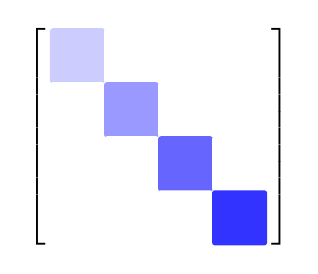
\begin{tikzpicture}[node distance=2.0cm]
    \tikzset{
        gridMatrix/.style={
            matrix of nodes,
            nodes={
                minimum size=0.7cm,
                anchor=center,
                inner sep=0pt,
                font=\tiny
            },
            column sep=-\pgflinewidth,
            row sep=-\pgflinewidth,
            nodes in empty cells,
            inner sep=0pt,
            rounded corners=1pt
        }
    }
    \matrix[gridMatrix, left delimiter={[}, right delimiter={]}] (diag) {
        |[fill=blue!20]| {} & |[fill=white]| {} & |[fill=white]| {} & |[fill=white]| {} \\
        |[fill=white]| {} & |[fill=blue!40]| {} & |[fill=white]| {} & |[fill=white]| {} \\
        |[fill=white]| {} & |[fill=white]| {} & |[fill=blue!60]| {} & |[fill=white]| {} \\
        |[fill=white]| {} & |[fill=white]| {} & |[fill=white]| {} & |[fill=blue!80]| {} \\
    };
\end{tikzpicture}
\end{adjustbox}
\end{minipage}
\end{adjustbox}
\hspace{10.3mm}
\begin{adjustbox}{width=0.32\textwidth}
\begin{minipage}[c]{0.335\linewidth} %
\begin{adjustbox}{width=1.0\textwidth}
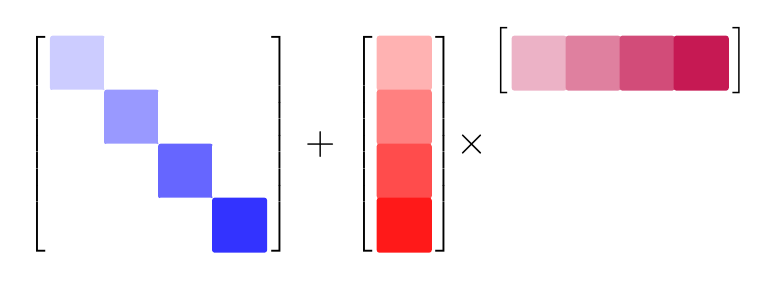
\begin{tikzpicture}[node distance=2cm]
    \tikzset{
        gridMatrix/.style={
            matrix of nodes,
            nodes={
                minimum size=0.7cm,
                anchor=center,
                inner sep=0pt,
                font=\tiny
            },
            column sep=-\pgflinewidth,
            row sep=-\pgflinewidth,
            nodes in empty cells,
            inner sep=0pt,
            rounded corners=1pt
        }
    }
    \matrix[gridMatrix, left delimiter={[}, right delimiter={]}] (diag) {
        |[fill=blue!20]| {} & |[fill=white]| {} & |[fill=white]| {} & |[fill=white]| {} \\
        |[fill=white]| {} & |[fill=blue!40]| {} & |[fill=white]| {} & |[fill=white]| {} \\
        |[fill=white]| {} & |[fill=white]| {} & |[fill=blue!60]| {} & |[fill=white]| {} \\
        |[fill=white]| {} & |[fill=white]| {} & |[fill=white]| {} & |[fill=blue!80]| {} \\
    };
    \node[right=0.35cm of diag] (plus) {\Large $+$};
    \matrix[gridMatrix, left delimiter={[}, right delimiter={]}] (colVec) 
       at ($(plus.east)+(0.75,0)$) {
        |[fill=red!30]| {} \\
        |[fill=red!50]| {} \\
        |[fill=red!70]| {} \\
        |[fill=red!90]| {} \\
    };
    \node at ($(colVec.east)!0.5!(colVec.east)+(0.5,0)$) {\Large $\times$};
    \matrix[gridMatrix, left delimiter={[}, right delimiter={]}, anchor=north west, baseline=0.3cm]
       (rowVec) at ($(colVec.north east)+(1.0cm,0)$) {
        |[fill=purple!30]| {} & |[fill=purple!50]| {} & |[fill=purple!70]| {} & |[fill=purple!90]| {} \\ 
        |[fill=white, opacity=0, minimum size=0.05cm]| {} & |[fill=white, opacity=0, minimum size=0.05cm]| {} & |[fill=white, opacity=0, minimum size=0.05cm]| {} & |[fill=white, opacity=0, minimum size=0.05cm]| {} \\
    };
\end{tikzpicture}
\end{adjustbox}
\end{minipage}
\end{adjustbox}
\hspace{3.6mm}
\begin{adjustbox}{width=0.36\textwidth}
\begin{minipage}[c]{0.355\linewidth} %
\vspace{5.5mm}
\begin{adjustbox}{width=1.0\textwidth}
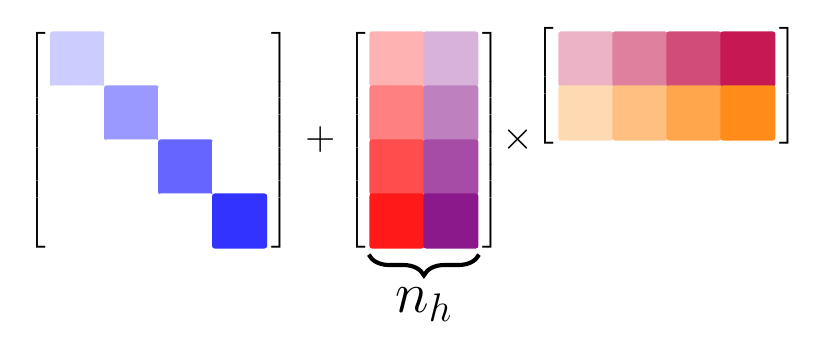
\begin{tikzpicture}[node distance=2cm]
    \tikzset{
        gridMatrix/.style={
            matrix of nodes,
            nodes={
                minimum size=0.7cm,
                anchor=center,
                inner sep=0pt,
                font=\tiny
            },
            column sep=-\pgflinewidth,
            row sep=-\pgflinewidth,
            nodes in empty cells,
            inner sep=0pt,
            rounded corners=1pt
        }
    }
    \matrix[gridMatrix, left delimiter={[}, right delimiter={]}] (diag) {
        |[fill=blue!20]| {} & |[fill=white]| {} & |[fill=white]| {} & |[fill=white]| {} \\
        |[fill=white]| {} & |[fill=blue!40]| {} & |[fill=white]| {} & |[fill=white]| {} \\
        |[fill=white]| {} & |[fill=white]| {} & |[fill=blue!60]| {} & |[fill=white]| {} \\
        |[fill=white]| {} & |[fill=white]| {} & |[fill=white]| {} & |[fill=blue!80]| {} \\
    };
    \node[right=0.35cm of diag] (plus) {\Large $+$};
    \matrix[gridMatrix, left delimiter={[}, right delimiter={]}] (colVec) 
       at ($(plus.east)+(1.0,0)$) {
        |[fill=red!30]| {} & |[fill=violet!30]| {} \\
        |[fill=red!50]| {} & |[fill=violet!50]| {} \\
        |[fill=red!70]| {} & |[fill=violet!70]| {} \\
        |[fill=red!90]| {} & |[fill=violet!90]| {} \\
    };
    \draw[decorate, decoration={brace, mirror, amplitude=7.5pt, raise=2pt, aspect=0.5pt}, line width=1.5pt]
        (colVec.south west) -- (colVec.south east)
        node[midway, below=10pt] {\huge $n_h$};
    \node at ($(colVec.east)!0.5!(colVec.east)+(0.5,0)$) {\Large $\times$};
    \matrix[gridMatrix, left delimiter={[}, right delimiter={]}, anchor=north west, baseline=0.3cm]
       (rowVec) at ($(colVec.north east)+(1.0cm,0)$) {
        |[fill=purple!30]| {} & |[fill=purple!50]| {} & |[fill=purple!70]| {} & |[fill=purple!90]| {} \\ 
        |[fill=orange!30]| {} & |[fill=orange!50]| {} & |[fill=orange!70]| {} & |[fill=orange!90]| {} \\
        |[fill=white, opacity=0, minimum size=0.05cm]| {} & |[fill=white, opacity=0, minimum size=0.05cm]| {} & |[fill=white, opacity=0, minimum size=0.05cm]| {} & |[fill=white, opacity=0, minimum size=0.05cm]| {} \\
    };
\end{tikzpicture}
\end{adjustbox}
\end{minipage}
\end{adjustbox}
\end{adjustbox} \\

\vspace{-1mm}
\begin{minipage}[b]{0.13\linewidth}
{\footnotesize
    \textcolor{white}{Diagonal}\\
    \textit{Token Mix:} \\
    \textit{Channel Mix:}\\
    \textit{Expressivity:}\\
    \textit{Examples: }}
    \end{minipage}
\begin{minipage}[b]{0.16\linewidth}
{\footnotesize
    \textbf{Diagonal:}\\
    $\checkmark$ \\
    $\times$ \\
    Parity \\
    Mamba, GLA}
    \end{minipage}
\hspace{2.0mm}
\begin{minipage}[b]{0.23\linewidth}
{\footnotesize
    \textbf{Rank 1 Update:}\\
    $\checkmark$ \\
    $\checkmark$ \\
    Reflections \\
    DeltaNet, TTT, RWKV-7}
    \end{minipage}
\hspace{13.5mm}
\begin{minipage}[b]{0.2\linewidth}
{\footnotesize
\textbf{Rank $n_h$ Update:}\\
$\checkmark$ \\
$\checkmark$ \\
Reflections, Rotations \\
\textbf{DeltaProduct}}
\end{minipage}
\vspace{-2mm}
\caption{Overview of state-transition matrices in linear RNNs: Diagonal matrices (e.g., in Mamba/mLSTM) mix tokens only; rank‑1 updates (DeltaNet/TTT) mix tokens and channels; and our proposed DeltaProduct performs rank‑\(n_h\) updates, further increasing the expressivity.}
\label{fig:rank_update_overview}
\end{figure}

\vspace{-3mm}
In this work, we propose \textit{DeltaProduct}, a generalization of DeltaNet that enhances its expressivity by featuring state transition matrices formed as a product of generalized Householder matrices. 
While DeltaNet's recurrence can be seen as performing one step of online gradient descent per token, DeltaProduct further refines the hidden state update \emph{multiple times per token}, naturally leading to a more expressive state-transition matrix, where each additional step expands the range of achievable linear transformations.

Formally, for each input token $x_i$ to the layer we generate $n_h$ keys as $\vk_{i,j}$ = $\mW_j \vx_i/\lVert \mW_j \vx_i \rVert_2$, $n_h$ values as $\vv_{i,j} = \mV_j \vx_i$, and $n_h$ betas as $\beta_{i,j} = \phi(\mU_j \vx_i)$  where $\mW_j, \mV_j, \mU_j$,  are learnable weight matrices specific to the $j$-th gradient step, while $\phi$ is either the sigmoid or $2 \times$ the sigmoid as suggested by \citet{grazzi-iclr25a} to increase the expressivity and state-tracking capabilities. Then, we compute $n_h$ gradient descent steps using the losses $\mathcal{L}_{i,j}(\mH) =\|\mH^\top\vk_{i,j} - \vv_{i,j}\|_2^2/2$, i.e.\@ for $j=1\dots n_h$
\begin{align*}
    \mH_{i, j} =  \mH_{i,j-1} - \beta_{i, j} \nabla \mathcal{L}_{i,j}(\mH_{i,j-1})  
    = \left(\mI - \beta_{i, j} \vk_{i, j} \vk_{i, j}^\top\right) \mH_{i,j-1} + \beta_{i, j} \vk_{i, j} \vv_{i, j}^\top,
\end{align*}
where $\mH_{i,0} = \mH_{i-1}$ and $\mH_{i, n_h} = \mH_i$. Unrolling, we get $\mH_i = \mA(\vx_i) \mH_{i-1} + \mB(\vx_i)$ with
\begin{tcolorbox}[
  colback=white!3!white,
  colframe=red,
  boxrule=0.5pt,
  arc=2mm,
  left=1mm,
  right=1mm,
  top=-2.6mm,
  bottom=0mm]
\[
\mA(\vx_i) = \prod_{j=1}^{n_h} \Bigl(\mI - \beta_{i,j}\,\vk_{i,j}\vk_{i,j}^\top\Bigr), \quad
\mB(\vx_i) = \sum_{j=1}^{n_h} \Bigl(\prod_{k=j+1}^{n_h} \bigl(\mI - \beta_{i,k}\,\vk_{i,k}\vk_{i,k}^\top\bigr)\Bigr)\,\beta_{i,j}\,\vk_{i,j}\vv_{i,j}^\top.
\]
\end{tcolorbox}

Hence, by taking multiple gradient descent steps per token, DeltaProduct's state-transition matrices are \textit{products of generalized Householder transformations}, and by expanding such product, $\mA(\vx_i)$ takes the form of identity plus a matrix of rank at most $n_h$ as shown in~\Cref{fig:rank_update_overview}. 
This formulation enables DeltaProduct to interpolate between generalized Householder ($n_h = 1$ as in DeltaNet) and dense 
matrices, since increasing $n_h$ increases the rank of the update performed on the hidden state.

An important consequence of using Householder products is that it allows us to efficiently bound the norm of $\mA(\vx_i)$, since the norm of the product is upper bounded by the product of the norms (each $\leq 1$), ensuring the stability of the recurrence. %
This bound would not be possible with a  the direct formulation $\mA(\vx_i) = I - \sum_{j=1}^{n_h} \beta_{i,j}\vk_{i,j}\vk_{i,j}^\top$, which would also restrict the matrix to be symmetric.
Notably, for each layer, DeltaProduct uses $n_h$ distinct key projection matrices to generate different keys $\vk_{i,1},\dots, \vk_{i,n_h}$ for the same input token. This ability to generate multiple, potentially orthogonal keys is essential for enhancing the recurrence's expressivity beyond DeltaNet. For instance, if we were to use identical keys across steps, the product of generalized Householders would collapse into a single generalized Householder transformation with a scaled $\beta$ (see Lemma~\ref{lemma:product_rank1_same_direction}). Just as DeltaNet extends to Gated DeltaNet by incorporating a forget gate~\citep{yang-iclr25a}, DeltaProduct can similarly be extended to Gated DeltaProduct (see~\Cref{app:gated_delta_product} for details).


\textbf{Implementation.}  
Since each step of DeltaProduct follows the same recurrence structure as DeltaNet, we can reuse its recurrence implementation written in Triton~\citep{tillet2019triton}, which is available through the \textsc{Flash-Linear-Attention} library~\citep{yang2024fla}. However, DeltaProduct differs by using $n_h$ keys and values per token, resulting in a recurrence $n_h$ times longer than DeltaNet's. For a sequence of length \( l \) with \( n_h \) Householders, the keys (and similarly the values and betas) are arranged as:  
$
\left[\mathbf{k}_{1,1}, \ldots, \mathbf{k}_{1,n_h}, \mathbf{k}_{2,1}, \ldots, \mathbf{k}_{2,n_h}, \ldots \right].
$
For gating, we multiply a scalar gate to the state transition matrix, as in Gated DeltaNet~\citep{yang-iclr25a}, using a single gate \( g_i \in \mathbb{R}\) per token \( \mathbf{x}_i \), structured as:  
$
\left[ g_1, 1, \ldots, 1, g_2, 1, \ldots, 1, \ldots \right]
$ 
where each \( g_i \) is followed by \( (n_h-1) \) ones to match the number of keys and values. Once the recurrence is evaluated, we keep only every $n_h$-th element of the output,
so that the output sequence retains the same length as the input sequence. Note that the runtime of DeltaProduct scales linearly with $n_h$ as demonstrated in~\Cref{app:runtime}.

\textbf{Theoretical Expressivity.}
As shown by \citet[Theorem 3 and 4]{grazzi-iclr25a}, a linear RNN with state-transition matrices parameterized as the product of $n_h$ generalized Householder transformations (whose eigenvalues lie in $[-1,1]$) can solve any group word problem with state-transitions limited to permutations of at most $n_h + 1$ elements in one layer. Moreover, multiple layers allow it to recognize any regular language with sufficiently large $n_h$.
Hence, by increasing \(n_h\), DeltaProduct provides a tunable mechanism to control the expressivity of the recurrence, making it particularly effective for tasks requiring complex state tracking. Moreover, since each Householder transform is weighted by a coefficient \(\beta_{i,j}\), the model can learn to set specific \(\beta_{i,j}\) values to zero when processing certain tokens. This adaptively ``skips'' one or more gradient steps, effectively allowing the network to modulate compute on a token-by-token basis, thereby providing a route toward dynamic computation, reminiscent of ACT~\citep{graves2016adaptive}. 
\vspace{-5pt}
\section{Two Layer DeltaNet Can Solve Dihedral group Word Problems}
\label{sec:dihedral_theory}
\vspace{-7pt}
In contrast to increasing the number of gradient steps per token, the expressivity of DeltaNet (equivalent to DeltaProduct with $n_h = 1$) can also be enhanced by increasing the number of layers and its theoretical limit is still unknown. In \citet[Theorem 6]{grazzi-iclr25a} it is shown that  with 2 layers and the extended eigenvalue range, DeltaNet can compute addition modulo $m$, which corresponds to solving the group word problem for the cyclic group $\mathbb{Z}_m$, for any $m \in \N$.



We extend \citet[Theorem 6]{grazzi-iclr25a} to prove that, under identical assumptions, DeltaNet can solve the group word problem for the dihedral group $D_m$, for any $m \in \N$. The dihedral group $D_m$ represents the symmetries (both rotations and reflections) of a regular $m$-sided polygon. As a notable example, $D_3$ is isomorphic to the symmetric group $S_3$. The linear RNN construction used in this result can be implemented using a 2-layer DeltaNet Model with two heads in the first layer.

\begin{theorem}[Dihedral group word problems with reflections]\label{thm:dihedral} A finite precision linear RNN with two layers in the form (\ref{eq:linrnn}), where in the first layer $\mA(\vx_t) = \mathrm{diag}(\va(\vx_t))$, with $\va(\vx_t) \in \{1,-1\}^2$ and in the second layer $\mA(\vx_t) \in \mathcal{H} \subset \R^{2 \times 2}$ where $\mathcal{H} = \{I - 2 \vv\vv^\top : \vv \in \R^2, \lVert \vv \rVert =1 \}$ is the set of all 2D reflections, can solve the group world problem of the dihedral group $D_m$ for any $m\in N$. 
\end{theorem}
The complete proof is provided in \Cref{sec:proof} and uses the following construction. In the first layer, the linear RNN will compute parity for rotations and reflections separately, i.e. it will record if the number of past rotations (reflections) is even or odd. 
The recurrent state of the second layer will have $2m$ possible values (same as the order of $D_m$) and each will be decoded differently based on the parity of reflections. 
The parity of rotations, combined with the group element, determines which reflection matrix to use as the state transition matrix of the second layer.

\vspace{-10pt}
\section{Experiments}\label{sec:experiments}
\vspace{-5pt}
We evaluate DeltaProduct on a range of tasks—from state-tracking and chomsky hierarchy problems to standard language modeling—to assess its expressivity and efficiency. In each experiment, unless otherwise specified, we vary the number of Householder transformations per token ($n_h$) while keeping other parameters fixed, thereby trading-off increased computational cost and parameter count for enhanced expressivity. Throughout the experiments we use either the suffix $[-1,1]$ or $[0,1]$ after each method, to denote the eigenvalue ranges of its state transition matrices.
\vspace{-5pt}
\subsection{State-Tracking}\label{sec:state-tracking}

\begin{figure}
    \centering
    \adjustbox{width=1.0\textwidth}{
    \includegraphics[width=0.2405\textwidth, trim={4 26 3 0}, clip=true] {figures/state_tracking/S3.pdf}
    \includegraphics[width=0.195\textwidth, trim={30 26 3 0}, clip=true] {figures/state_tracking/S4.pdf}
    \includegraphics[width=0.195\textwidth, trim={30 26 3 0}, clip=true] {figures/state_tracking/A5.pdf}
    \includegraphics[width=0.195\textwidth, trim={30 26 3 0}, clip=true] {figures/state_tracking/S5.pdf}
    }
        \adjustbox{width=1.0\textwidth}{
    \includegraphics[width=0.2405\textwidth, trim={4 0 3 18}, clip=true] {figures/state_tracking_layers/S3.pdf}
    \includegraphics[width=0.195\textwidth, trim={30 0 3 18}, clip=true] {figures/state_tracking_layers/S4.pdf}
    \includegraphics[width=0.195\textwidth, trim={30 0 3 18}, clip=true] {figures/state_tracking_layers/A5.pdf}
    \includegraphics[width=0.195\textwidth, trim={30 0 3 18}, clip=true] {figures/state_tracking_layers/S5.pdf}
    }
    \vspace{-8mm}
    \caption{Accuracy on state-tracking tasks for permutation groups \( S_3 \), \( S_4 \), \( A_5 \), and \( S_5 \), plotted against sequence length (x-axis). \textit{(Top row)} Varying the number of Householder products \(n_h \) for a single layer DeltaProduct$_{n_h}[-1,1]$. \textit{(Bottom row)} Varying the number of layers $l$ of DeltaProduct$_{1}[-1,1]$/DeltaNet$[-1,1]$ (single Householder). Dashed vertical line at training context length 128. Higher \( n_h \) improves extrapolation to longer sequences of permutations, e.g., \( S_3 \) can be learned with \( n_h=2 \) with a single layer while three layers are required when keeping $n_h=1$.
    } 
    \vspace{-5pt}\label{fig:state_tracking_length_extrapolation}
\end{figure}

\begin{wrapfigure}[17]{r}{0.26\linewidth}
  \centering
  \vspace{-5mm}
  \adjustbox{width=\linewidth}{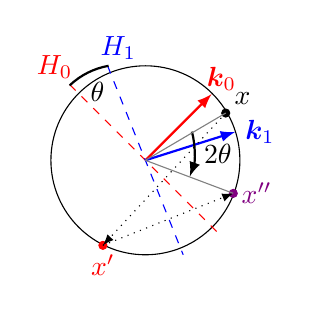
\begin{tikzpicture}[>=latex, scale=1.2,
                    every label/.style={font=\scriptsize},
                    annotation/.style={font=\scriptsize, align=center}]

  
  \draw (0,0) circle (1);

  \draw[dashed,red] (-0.8,0.8) -- (0.8,-0.8)
    node[pos=0.3, above left, xshift=-4.2mm, yshift=5.3mm] {$H_0$};

  \draw[dashed,blue] (-0.4,1) -- (0.4,-1)
    node[pos=0.3, above right, xshift=-5mm, yshift=6.7mm] {$H_1$};

  \draw[->,thick,red] (0,0) -- (0.7,0.7)
    node[above left=-3mm, xshift=2.3mm, yshift=1.3mm] {$\vk_0$};
  \draw[->,thick,blue] (0,0) -- (0.95,0.3)
    node[right=0mm] {$\vk_1$};

  \draw[-,thick,black!50!black] (-0.39, 1.0) arc (100:133.5:0.8)
    node[pos=0.2, right, xshift=-2.5mm, yshift=-3mm] {$\theta$};
  
  \draw[<-,thick,black!50!black] ({0.5*cos(-20)},{0.5*sin(-20)}) 
      arc (-20:14.5:0.8)
      node[pos=0.5, above, xshift=3mm, yshift=-2.5mm] {$2\theta$};

  \coordinate (X) at (0.85,0.5);
  \draw[fill] (X) circle (1.2pt) node[above right=-0.5pt] {$x$};

  \coordinate (X') at  (-0.45,-0.9);
  \draw[fill, red] (X') circle (1.2pt) node[below] {$x'$};
  \draw[dotted,->] (X) -- (X'); 

  \coordinate (X'') at (0.93,-0.35);
  \draw[fill, violet] (X'') circle (1.2pt) node[below, right=-0.5pt] {$x''$};
  \draw[dotted,->] (X') -- (X''); 
  \draw[gray] (0,0) -- (X);

\draw[gray] (0,0) -- (X'');

\end{tikzpicture}}
  \vspace{-7 mm}
  \caption{Two reflections produce a rotation: Reflecting \(x\) across planes \(H_0\) and \(H_1\) (with normals \(\vk_0\) and \(\vk_1\)) yields a rotation by \(2\theta\), where \(\theta\) is the angle between the planes.}
  \label{fig:rotation}
\end{wrapfigure}
\textbf{Setup.} 
We evaluate DeltaProduct's ability to capture complex state dynamics using group word problems of increasing difficulty, specifically on the permutation groups \( S_3\), \( S_4\), \( A_5\), and \( S_5\), as implemented by~\citet{merrill-icml24a}. We train on sequences of up to 128 products of permutations/tokens in length and subsequently measure extrapolation on sequences of up to 512 tokens. Throughout, we use the extended setting, allowing eigenvalues in \([-1,1]\). DeltaProduct models failed to learn even the training context-length when restricted to the standard eigenvalue range $[0, 1]$, regardless of the number of Householder transformations $n_h$ 
and so we omit the results. See~\Cref{app:state_tracking} for details on the experimental setup.

\textbf{Results.} \Cref{fig:state_tracking_length_extrapolation} (top row) demonstrates the benefits of increasing the number of gradient steps \(n_h\) per token for a single layer DeltaProduct. In agreement with \citet[Theorem 3]{grazzi-iclr25a}, for \(S_3\), achieving reliable performance beyond sequence lengths of 128 requires \(n_h=2\), while \(S_5\) needs \(n_h=4\). Unexpectedly, \(S_4\) and \(A_5\) can extrapolate robustly using only \(n_h=2\) despite the theorem suggesting 3 and 4 respectively. This efficiency arises from their isomorphism to subgroups of \(\mathrm{SO}(3,\mathbb{R})\) \citep[Ch. 1, Sec. 2.4]{schwarzbach2010groups}: each element can be mapped to a 3D rotation via just two Householder reflections (see \Cref{fig:rotation}); a consequence of the Cartan-Dieudonné theorem~\citep{springer_cartan} stating that any orthogonal transformation (e.g. rotations) can be expressed as a composition of reflections. See~\Cref{app:state_tracking} for details on the isomorphisms of $S_4$, $A_5$, and $S_5$. 

In \Cref{fig:state_tracking_length_extrapolation} (bottom row), we explore the limits of the expressivity of DeltaNet (i.e. $n_h=1$) with multiple layers, which is still not fully understood theoretically. Increasing the number of layers while keeping $n_h=1$ improves performance but less effectively than increasing $n_h$. Interestingly, DeltaNet cannot learn $S_4$ and $S_5$ even with 5 layers, and with two layers, it performs poorly also on $S_3$, even though \Cref{thm:dihedral} shows that it can solve it. This suggests that simply increasing the number of layers may not be sufficient to attain the improvements of DeltaProduct enabled by incorporating more Householder transformations.

\textbf{Analysis.} To empirically validate whether DeltaProduct$_2[-1,1]$ exploits the isomorphism of $S_4$ to subgroups of $\mathrm{SO}(3,\mathbb{R})$, we verified two hypotheses: whether both householders act as reflections ($\beta_0=\beta_1=2$) composing to form rotations, and whether the keys exist in a three-dimensional subspace. By recording $\beta_0$ and $\beta_1$ values (representing the first and second householder in the product) across all 24 permutations of $S_4$, we find that a single head had indeed learned to use both Householder transformations as reflections where $\beta_0=\beta_1=2$, effectively creating rotation matrices as shown in Figure \ref{fig:app_beta_values_estimated}. 
This pattern is evident in Figure \ref{fig:S4_beta_inv} (left), where this head consistently displays beta values of approximately 2, confirming that the model successfully learns to 
\begin{wrapfigure}[14]{r}{0.535\linewidth}
  \centering
  \vspace{-3mm}
  \adjustbox{width=\linewidth}{
  \includegraphics[width=0.423\linewidth, trim={3.5 0 0 0}, clip=true]{figures/state_tracking/beta_outputs_bootstrap_stats_S4_512.pdf}
  \includegraphics[width=0.51\linewidth, trim={0 0 3 0}, clip=true]{figures/state_tracking/full_X_full.pdf}}
  \vspace{-7mm}
  \caption{\emph{(Left)} Estimated beta values for DeltaProduct$_2[-1,1]$ on all permutations of $S_4$, clustering near 2 (reflection). \emph{(Right)} PCA of key vectors shows that the first three components explain most of the variance.}
  \label{fig:S4_beta_inv}
\end{wrapfigure}approximate rotations by combining two reflections. 
To further verify whether the keys are in a three-dimensional subspace, we apply Principal Component Analysis (PCA)~\citep{pearson1901liii}  to the key vectors of the head where beta values approached 2. The results, displayed in Figure \ref{fig:S4_beta_inv} (right), demonstrate that three principal components account for over 95\% of the variance in the key space. This finding strongly supports our theoretical understanding, as it indicates that the model primarily operates in a three-dimensional subspace, which aligns with the structure of $\mathrm{SO}(3,\mathbb{R})$.
\subsection{Chomsky Hierarchy}\label{sec:chomsky}

\begin{wrapfigure}[12]{r}{0.425\linewidth}
  \centering
  \vspace{-5.1mm}
  \includegraphics[width=\linewidth, trim={3 2 8 0}, clip=true]{figures/chomsky/modular_arithmetic_with_brackets.pdf}
  \vspace{-8mm}
  \caption{Results on Modular Arithmetic with brackets: DeltaProduct $[-1, 1]$ consistently outperforms all other methods.}
  \label{fig:modular_arithmetic_with_bracket}
\end{wrapfigure}

\textbf{Setup.} We conducted experiments on selected formal language tasks originally introduced by \citet{deletang-iclr23a}. Our goal is to demonstrate the improvements in length extrapolation that can be achieved using multiple Householder matrices in the state-transition matrix compared to DeltaNet. Following \citet{grazzi-iclr25a}, we focus on three tasks: parity, modular arithmetic without brackets (both regular languages), and modular arithmetic with brackets (a context-free language). We trained DeltaProduct$_{n_h}$ with $n_h \in \{2,3,4\}$ on sequences of length 3 to 40 and tested on sequences ranging from 40 to 256 to evaluate generalization to longer inputs. We compare our results against Transformer, mLSTM and sLSTM from \citet{beck-neurips24a}, Mamba~\citep{gu2023mamba}, and DeltaNet~\citep{yang-neurips24a}. For both Mamba and DeltaNet, we experiment with eigenvalue ranges restricted to $[0,1]$ and extended to $[-1,1]$.


\textbf{Results.} 
 As shown in \Cref{tab:chomsky}, DeltaProduct$_{n_h}$ with $n_h \geq 2$ demonstrates greater expressivity compared to DeltaNet and other baselines. This performance improvement is particularly pronounced when using the extended eigenvalue range $[-1, 1]$, which aligns with the findings of \citet{grazzi-iclr25a}. Notably, we observe the most significant improvement in the modular arithmetic with brackets task, where DeltaNet$[-1,1]$ previously showed limitations~\citep{grazzi-iclr25a} (see~\Cref{fig:modular_arithmetic_with_bracket}). 
 Additional experimental details and hyperparameter values are provided in Appendix~\ref{app:chomsky}.
\subsection{Language Modeling}\label{sec:language_modelling}
\begin{table*}
\caption{Performance comparison using lm-eval-harness benchmark~\citep{eval-harness} (SlimPajama (SPJ) reproduced from~\citet{yang-neurips24a}, Fine-Web (FW) ours). Results are shown for DeltaProduct and Gated DeltaProduct. We use 8 heads for each layer, unless otherwise specified.
}
\vspace{1mm}
\centering
\adjustbox{width=0.98\textwidth}{
\centering
\begin{tabular}{c|l|cc|ccccccc|ccc}
\toprule
\textbf{} & \multirow{2}{*}{\hspace{5mm}\textbf{Model}}  & \textbf{Wiki.}  &  \textbf{LMB.} &  \textbf{LMB.} & \textbf{PIQA} &    \textbf{Hella.} & \textbf{Wino.} & \textbf{ARC-e} &  \textbf{ARC-c} &  \textbf{Avg.}  & \textbf{SWDE} & \textbf{SQUAD} & \textbf{FDA} \\
\textbf{} &  & ppl $\downarrow$  &  ppl $\downarrow$  &  acc $\uparrow$  & acc $\uparrow$ &   acc\_n $\uparrow$  & acc $\uparrow$  & acc $\uparrow$ & acc\_n $\uparrow$ & $\uparrow$ & cont. $\uparrow$  & cont. $\uparrow$ &  cont. $\uparrow$   \\
\midrule
\multirow{5}{*}{\rotatebox{90}{\scriptsize\textit{15B tokens SPJ}}} 
& \hspace{-1mm} {\textit{340M params}} & & & & & & & & & & & & \\
& \hspace{4mm} Transformer++ & \underline{28.39} & 42.69 & 31.0 & 63.3 & 34.0 & 50.4 & 44.5 & \underline{24.2} & 41.2  & \textbf{42.2} & 22.1 & \textbf{21.4} \\
& \hspace{4mm} Mamba  $[0, 1]$ & \underline{28.39} & \underline{39.66} & 30.6 & \underline{65.0} & \textbf{35.4} & 50.1 & \textbf{46.3} & 23.6 & \underline{41.8} & 12.4 & 23.0 & 2.1 \\ 
& \hspace{4mm} GLA $[0, 1]$ & 29.47 & 45.53 & \underline{31.3} & \textbf{65.1} & 33.8 & \underline{51.6} & 44.4 & \textbf{24.6} & \underline{41.8} & 24.0 & \underline{24.7} & 7.3 \\
& \hspace{4mm} DeltaNet $[0, 1]$ & \textbf{28.24} & \textbf{37.37} & \textbf{32.1} & 64.8 & \underline{34.3} & \textbf{52.2} & \underline{45.8} & 23.5 & \textbf{42.1} & \underline{26.4} & \textbf{28.9} & \underline{12.8}  \\ \midrule
\multirow{5}{*}{\rotatebox{90}{\scriptsize\textit{35B tokens FW~~~~~~}}} 
&DeltaNet$[-1,1]$ {\small 340M} & 26.92 & 43.07 & 29.8 & 69.0 & 41.0 & 50.9 & 46.6 & 24.5 & 43.6 & 26.4 & 30.2 & 3.7  \\
&DeltaNet$[-1,1]$ {\small 12 heads, 392M} & 26.57 & 36.76 & 31.8 & 69.2 & 42.3 & 50.9 & 47.2 & 24.4 & 44.3 & 15.8 & 11.0 & 0.18 \\
&DeltaProduct$_2[-1,1]$ {\small 392M } & 26.43 & 30.66 & \underline{34.0} & 68.9 & 42.4 & \underline{53.1} & 48.9 & \underline{25.9} & 45.5 & \textbf{32.0} & 30.0 & 3.9  \\
& DeltaProduct$_3[-1,1]$ {\small 443M} & 25.94 & \underline{29.91} & \underline{34.2} &  \textbf{69.9} & 43.2 & 51.9 &  48.2 & 24.1 & 45.2 & \underline{30.6} & \underline{30.4} & \underline{5.3} \\
\cmidrule(lr){2-14}
& Gated DeltaNet$[-1,1]$ {\small 340M} & 25.97 &  33.57 & 33.1 & \underline{69.5} & 44.1 & 51.1 & \textbf{50.9} & \textbf{26.7} & \underline{45.9} & 27.4 & 31.4 & 4.2 \\
& Gated DeltaProduct$_2[-1,1]$ {\small 393M} & \underline{25.12} & 30.03 & \underline{34.2} & 69.1 & \underline{44.6} & \textbf{55.3} & \underline{49.8} & 25.3 & \textbf{46.4} & 30.1 & \textbf{31.6} & \textbf{6.6}  \\

\bottomrule
\end{tabular}}
\label{table:lm-benchmarks}
\end{table*}

\begin{figure}[t]
    \centering\includegraphics[width=0.98\textwidth,trim={4 10 0 3}, clip=true]{figures/language_modelling/length_extrapolation/fw_35b/delta_net_340m/length_eval_seq_len_16384.pdf}
    \vspace{-2mm}
    \caption{Length extrapolation results for DeltaProduct$_{n_h}[-1,1]$ on long context datasets, where $n_h\in\{1,2,3\}$, tested on sequences up to 16,384 tokens. Solid and dashed lines represent models with 8 and 12 heads respectively. Note that DeltaProduct$_2[-1,1]$ with 8 heads (392M parameters) matches the parameter count of DeltaNet ($n_h=1$) with 12 heads, while achieving significantly better length extrapolation.}
\label{fig:deltaproduct_length_extrapolation}
\vspace{-2mm}
\end{figure}

\begin{wrapfigure}[23]{r}{0.3\linewidth}
\centering
\vspace{-12.6pt}
\adjustbox{width=\linewidth}{
\includegraphics[width=\linewidth, trim={4 0 0 20}, clip=true]{figures/language_modelling/scaling/scaling_train_perplexity.pdf}} \\
\adjustbox{width=\linewidth}{
\includegraphics[width=\linewidth, clip=true, trim={3 12 3 2}]{figures/language_modelling/scaling/scaling_downstream_reduced.pdf}}
\vspace{-21pt}
\caption{Scaling analysis of DeltaProduct$_{n_h}[-1, 1]$ (H=heads) w.r.t. final training perplexity on FineWeb (top), WikiText, and Lambada via lm-eval harness.}
\label{fig:scaling-plot}
\end{wrapfigure}
\textbf{Setup.} We trained two model variants: $\text{DeltaProduct}_{n_h}[-1, 1]$ and $\text{Gated DeltaProduct}_{n_h}[-1, 1]$ using the FineWeb dataset~\citep{penedo2024finewebdatasetsdecantingweb} with $35$B tokens. 
We adopted the training hyperparameters and pipeline of \citet{grazzi-iclr25a} (detailed in~\Cref{app:lm-experimental-setup}). We evaluated the models using language understanding, reasoning, and retrieval benchmarks from lm-eval-harness~\citep{eval-harness}, with task specifics in~\Cref{app:task_details}. To assess extrapolation, we measured perplexity beyond the training context length of 2048 tokens on CodeParrot~\citep{tunstall2022natural} for coding, OpenThoughts-114k-Math~\citep{openthoughts} for math, TriviaQA~\citep{2017arXivtriviaqa} for knowledge retrieval, and SlimPajama~\citep{cerebras2023slimpajama} for language modeling.

\textbf{Results.} 
Our experiments demonstrate that both DeltaProduct and Gated DeltaProduct on average outperform their baseline counterparts ($\text{DeltaNet}[-1,1]$ and $\text{Gated DeltaNet}[-1,1]$) across the considered language modeling benchmarks when we increase $n_h$, as shown in \Cref{table:lm-benchmarks}.
Interestingly, $\text{DeltaProduct}_{3}[-1,1]$ achieves comparable performance to $\text{Gated DeltaNet}[-1,1]$, despite lacking a forget gate mechanism - a component considered crucial for language modeling tasks~\citep{hochreiter1997long,gu2023mamba}.
Furthermore, our training process remained stable even as we increased the value of $n_h$ (see~\Cref{fig:training-curves}).
Remarkably, as shown in~\Cref{fig:deltaproduct_length_extrapolation}, DeltaProduct's length extrapolation performance increases significantly with higher $n_h$ values, and at $n_h=3$, the performance degradation is minimal across the sequence length (see also \Cref{fig:combined_length_extrapolation} for results up to 32k sequence length). We hypothesize that DeltaProduct achieves better length extrapolation by enhancing DeltaNet's forgetting mechanism. While DeltaNet requires $n$ rank-1 updates to reset its state to zero, DeltaProduct can accelerate this forgetting process by a factor of $n_h$. This improvement could allow DeltaProduct$_3[-1,1]$ to learn effective forgetting patterns during training without an additional scalar forget gate, unlike Gated DeltaNet.
With a head embedding dimension of 128, DeltaProduct$_3[-1,1]$ can reset its state in approximately 43 tokens, making it much more efficient at handling long-range dependencies. However, our experiments show that DeltaProduct$_2[-1,1]$ still performs better with a forget gate, as demonstrated by its improved results when compared to the non-gated version (see \Cref{fig:combined_length_extrapolation}). 
To fairly compare DeltaProduct and DeltaNet, we conducted scaling experiments that accounted for DeltaProduct's additional parameters from its extra key, value, and $\beta$ projection layers. We varied the number of heads in both models. As shown in~\Cref{fig:scaling-plot} (top), DeltaProduct consistently achieves better performance than DeltaNet, though the perplexity difference is modest.
We expanded our analysis by evaluating DeltaProduct$_2[-1,1]$ and DeltaNet across multiple benchmarks from lm-eval-harness~\citep{eval-harness}. 
The results, shown in~\Cref{fig:scaling-plot} (bottom), reinforce our findings from the fineweb dataset. DeltaProduct maintains its performance advantage on both WikiText and Lambada tasks, showing improved perplexity across all model configurations. 
Our results align with the findings from~\Cref{sec:state-tracking} on state tracking: adding more householders proves more effective for improving length extrapolation compared to increasing the number of heads/layers.
\section{Conclusion, Limitations, and Future Work}
We presented DeltaProduct, an extension of DeltaNet that uses products of Householder transformations as state-transition matrices. This approach bridges the gap between structured and dense matrices, with each recurrence step interpretable as multiple steps of gradient descent on an associative recall loss (compared to DeltaNet's single step). The number of Householder matrices ($n_h$) serves as a tunable parameter balancing expressivity and computational efficiency. Our experiments demonstrate DeltaProduct's superior performance over DeltaNet in state tracking, formal language recognition, and language modeling, with particularly strong length extrapolation results.
DeltaProduct represents a promising step toward developing sequence models that are both more capable while still remaining scalable.

\textbf{Limitations.} DeltaProduct has several key limitations. First, compared to DeltaNet, it requires more computational resources and memory, with requirements scaling linearly in $n_h$. Second, while both models can learn group word problems, we lack a comprehensive theoretical framework for understanding which problems can be learned when using multiple layers with relatively small values of $n_h$ (relative to the group's complexity).

\textbf{Future Work.} Future research could focus on integrating alternative matrix parametrizations, such as those used in RWKV-7, and identifying problems that DeltaProduct cannot solve under finite precision constraints, following the work by~\citet{sarrof-neurips24a} and~\citet{grazzi-iclr25a}. Finally, our DeltaProduct implementation could be further optimized through algorithmic improvements, such as those proposed in the recent work by~\citet{cirone2025parallelflow}.
\section*{Acknowledgements}
We would like to thank Songlin Yang and Eddie Bergman for constructive discussions. We acknowledge the support and assistance of the Data Science and Computation Facility and its Support Team, in particular Mattia Pini, in utilizing the IIT High-Performance Computing Infrastructure, on which we run part of our experiments.
This research was partially supported by the following sources:  PNRR MUR Project PE000013 CUP J53C22003010006 “Future Artificial Intelligence Research (FAIR)“, funded by the European Union – NextGenerationEU, and EU Project ELSA under grant agreement No. 101070617.
TAILOR, a project funded by EU Horizon 2020 research and innovation programme under GA No 952215; the Deutsche Forschungsgemeinschaft (DFG, German Research Foundation) under grant number 417962828; the European Research Council (ERC) Consolidator Grant 'Deep Learning 2.0' (grant no. 10). This research was partially funded by the Deutsche Forschungsgemeinschaft (DFG, German Research Foundation) under grant number 539134284, through EFRE (FEIH 2698644) and the state of Baden-Württemberg. Frank Hutter acknowledges financial support by the Hector Foundation. The authors acknowledge support from ELLIS and ELIZA. Funded by the European Union. The authors gratefully acknowledge the Gauss Center for Supercomputing eV (\url{www.gauss-centre.eu}) for funding this project by providing computing time on the GCS supercomputer JUWELS at Jülich Supercomputing Center (JSC). Views and opinions expressed are however those of the author(s) only and do not necessarily reflect those of the European Union or the ERC. Neither the European Union nor the ERC can be held responsible for them.
\vspace{-5pt}
\begin{figure}[h]
\begin{center}
\includegraphics[width=0.2\textwidth]{figures/BaWue_Logo_Standard_rgb_pos.png} ~~~ \includegraphics[width=0.2\textwidth]{figures/EN-Co-funded-by-the-EU_POS.png} 
\end{center}
\end{figure}

\bibliography{ref,bib/lib,bib/proc,bib/strings}
\bibliographystyle{iclr2025_conference}
\newpage
\appendix
\section{DeltaProduct with Identical Keys}


\begin{lemma}\label{lemma:product_rank1_same_direction}
  Let $\mathbf{k}\in\mathbb{R}^n$ be nonzero, and let 
  $\alpha_1,\dots,\alpha_m$ be real scalars. Then
  \[
     \prod_{j=1}^m 
     \bigl(\mathbf{I} \;-\; \alpha_j\, \mathbf{k}\mathbf{k}^\top \bigr)
     \;=\;
     \mathbf{I}
     \;-\;
     \alpha^*\,
     \mathbf{k}\mathbf{k}^\top
  \]
  for some real scalar $\alpha^*$ depending on $\{\alpha_j\}_{j=1}^m$. 
\end{lemma}

\begin{proof}
Without loss of generality, assume $\|\mathbf{k}\|=1$. Otherwise, factor out $\|\mathbf{k}\|$ to rescale each $\alpha_j$.

If $m=1$, then the statement is trivially satisfied with $\alpha^* = \alpha$.
Suppose the statement is true for $m \geq 1$, i.e.\@ 
\(
   \prod_{j=1}^m (\mathbf{I} - \alpha_j\, \mathbf{k}\mathbf{k}^\top)
   =
   \mathbf{I} - \alpha^{(m)}\,\mathbf{k}\mathbf{k}^\top.
\)
Multiplying by \((\mathbf{I} - \alpha_{m+1}\,\mathbf{k}\mathbf{k}^\top)\) produces
\[
   \mathbf{I} - \bigl[\alpha^{(m)} + \alpha_{m+1} - \alpha^{(m)}\alpha_{m+1}\bigr]
   \,\mathbf{k}\mathbf{k}^\top.
\]
Hence, by induction, the product of any number of such factors remains of the form 
\(\mathbf{I} - \alpha^* \mathbf{k}\mathbf{k}^\top\).
\end{proof}


\section{Gated DeltaProduct}
\label{app:gated_delta_product}

When adapting the Gated DeltaNet approach to Gated DeltaProduct, we define the state-transition matrices \( \mA \) and input matrices \( \mB \) as follows:
\[
\mA(\vx_i) = \textcolor{red}{g_i} \prod_{j=1}^{n_h} \Bigl(\mI - \beta_{i,j}\,\vk_{i,j}\vk_{i,j}^\top\Bigr), \quad
\mB(\vx_i) = \sum_{j=1}^{n_h} \Bigl(\prod_{k=j+1}^{n_h} \bigl(\mI - \beta_{i,k}\,\vk_{i,k}\vk_{i,k}^\top\bigr)\Bigr)\,\beta_{i,j}\,\vk_{i,j}\vv_{i,j}^\top.
\]
where the gating term \( g_i \) is computed as:
\[
g_i = \text{sigmoid}(\vw_g \vx_i) \in [0, 1],~\vw_g\in \mathbb{R}^l
\]


\section{Runtime of DeltaProduct}\label{app:runtime}
\begin{figure}[ht]
    \centering
    \includegraphics[width=0.4\linewidth]{figures/runtime/fully_fused_gated_delta_product_varying_householders.pdf}
    \caption{\textit{DeltaProduct$_{n_h}$ scales linearly with $n_h$}. Runtime analysis of a single layer of DeltaProduct.}
    \label{fig:runtime}
\end{figure}

We evaluate the DeltaProduct layer on sequence lengths logarithmically spaced between 64 and 8192, while varying the number of Householder reflections from 1 to 4. Experiments were conducted on an Nvidia L40 GPU using \texttt{bfloat16} precision with a fixed batch size of 4. For each configuration, the model was run for 200 iterations and the runtimes were averaged following a burn-in phase of 3 iterations. The model was configured with a hidden size of 1024, a head dimension of 128 with 8 attention heads, and an expansion factor of 1.0. All models were compiled using \texttt{torch.compile} to ensure optimized performance. At a sequence length of 8192, the Delta Product layer achieved runtimes of approximately 0.006 seconds for 1 Householder, 0.010644 seconds for 2 Householder reflections, 0.01527 seconds for 3, and 0.01986 seconds for 4, respectively. These results, as shown in~\Cref{fig:runtime}, provide empirical evidence that the runtime increases linearly with the number of householders, since the computational cost scales as $n_h$ times the sequence length.



\section{Proof of \Cref{thm:dihedral}}\label{sec:proof}

\begin{proof}
The elements of the dihedral group $D_m$ can be divided into $m$ rotations $\mathcal{R} =\{r_0, \dots, r_{m-1}\}$ and $m$ reflections $\mathcal{S} =\{s_0, \dots, s_{m-1}\}$. The identity is $r_0$. To be able to solve the corresponding word problem, we would like to map sequences of group elements $x_1,\dots, x_t$ with $x_i \in \mathcal{R}\cup\mathcal{S}$ into sequences $y_1,\dots, y_t$ with $y_i = x_1 \cdot x_2 \cdots x_i$ and $\cdot$ is the group operation, that for dihedral groups is defined as
\begin{equation}\label{eq:groupop}
    r_i \cdot r_j=r_{i+j \bmod m}, \quad r_i \cdot s_j=s_{i+j \bmod m}, \quad s_i \cdot r_j=s_{i-j \bmod m}, \quad s_i \cdot s_j=r_{i-j \bmod m}.
\end{equation}
Note that a product of two rotations is commutative, while the product of two reflections or a reflection with a rotation is not. Indeed for $m \geq 3$ $D_m$, is not an abelian group.

The constructions of the two layers of the linear RNN builds upon the one for the cyclic group $Z_m$ outlined in \citep[Theorem 6]{grazzi-iclr25a}. The first layer is constructed to output parity separately for rotations and reflections. In particular, using the following diagonal recurrence which indicates in the first (second) coordinate whether the number of rotations (reflections) is even (0) or odd (1). 
\begin{gather*}
\vh^{(1)}_{0} = 0, \quad  \vh_{t}^{(1)} = \va(x_t) \odot \vh^{(1)}_{t-1} + \vb(x_t), \quad \vy^{(1)}_t = \mathrm{dec}^{(1)}(\vh_{t}, x_t) = (x_t, h_{t,1}, h_{t,2}). \\
\va(x_i)_1 = \begin{cases}
-1 & \text{if } x_i \in \mathcal{R}    \\
1 & \text{if } x_i \in \mathcal{S}
\end{cases} \quad \va(x_i)_2 = \begin{cases}
-1 & \text{if } x_i \in \mathcal{S}    \\
1 & \text{if } x_i \in \mathcal{R}
\end{cases} \\
\vb(x_i)_1 = \begin{cases}
1 & \text{if } x_i \in \mathcal{R}    \\
0 & \text{if } x_i \in \mathcal{S}
\end{cases} \quad \vb(x_i)_2 = \begin{cases}
1 & \text{if } x_i \in \mathcal{S}    \\
0 & \text{if } x_i \in \mathcal{R}
\end{cases} \\
\end{gather*} 
This recurrence can be implemented also by DeltaNet, which uses generalized Householder matrices, but it requires at least 2 heads.
For the second layer, we have instead the following constructions, which selects the appropriate reflection based on the parity of the rotations and uses the parity of the reflections for $\mathrm{dec}$.
\begin{gather*}
    \vh^{(2)}_{0} = (1,0)^\top, \quad  \vh^{(2)}_t = \mA^{(2)}(\vy^{(1)}_t) \vh^{(2)}_{t-1}, \quad \vy^{(2)}_t = \mathrm{dec}^{(2)}(\vh_t^{(2)}, \vy^{(1)}_t)  \\
    \mA^{(2)}(\vy) = \mH(\theta(y_1, y_2)) = \left[\begin{array}{cc}
\cos \theta(y_1, y_2) &  \sin \theta(y_1, y_2) \\
\sin \theta(y_1, y_2, ) & -\cos \theta(y_1, y_2)
\end{array}\right] \\
    \mathrm{dec}^{(2)}(\vh, \vy) = \begin{cases} 
    r_{i^*} & \text{if } y_3 = 0 \\
    s_{m-i^*} & \text{if } y_3 = 1
    \end{cases}, \quad 
    i^* = \argmax_{i \in \{0, \dots, m-1\}} \max (\vc_i^\top \vh, \vd_i^\top \vh) \quad 
\end{gather*}
where $\vy = (y_1, y_2, y_3)^\top \in \mathcal{R}\cup\mathcal{S} \times \{0,1\} \times \{0,1\}$,  $\mH(\alpha)$ is the $2 \times 2$ reflection matrix that reflects all vectors by a line having an angle of $\alpha/2$ with the line passing from the origin and the vector $(1,0)^\top$ and $\theta:  \mathcal{R}\cup\mathcal{S} \times \{0,1\} \to \R$ determines the angle of the reflection and is defined for all $i \in \{0,\dots, m-1\}$ as
\begin{align*}
    \theta(r_i, 1) &= \frac{(1 - 2i)\pi}{m}, \quad
    \theta(r_i, 0) = \frac{(1+2i) \pi}{m}, \quad  %
    \quad \theta(s_j, 1) = \frac{ - 2i\pi}{m}, \quad
    \theta(s_i, 0) = \frac{(2+2j) \pi}{m}. %
\end{align*} 
Moreover, $\mathcal{C} = \{\vc_0,\dots, \vc_{m-1}\}$ and $\mathcal{D} = \{\vd_0,\dots, \vd_{m-1}\}$ are two sets of states and are defined as
\begin{gather*}
\vd_0 = \vh_0^{(2)} =  (1,0)^\top, \quad \vc_0 = \mH(\pi/m)\vd_0, \\ \vd_i = \mR(2i\pi/m) \vd_0, \quad \vc_i = \mR(-2i\pi/m)\vc_0 \quad    \text{for all } i \in \{0,\dots,  m-1\},
\end{gather*}
where $\mR(\beta)$ is a rotation matrix with angle $\beta \in \R$.  

Let $\alpha,\gamma \in \R$, the following are standard identities of products of 2D rotations and reflections.
\begin{align*}
\begin{aligned}
\mR(\alpha) \mR(\gamma) & =\mR(\alpha + \gamma), \quad 
 &&\mH(\alpha)\mH(\gamma)  =\mR(\alpha- \gamma), \\
\mR(\alpha) \mH(\gamma) & =\mH\left(\alpha+ \gamma\right) 
&&\mH(\gamma) \mR(\alpha)  =\mH\left(\gamma-\alpha\right).
\end{aligned}
\end{align*}
From our choice of $\vd_0 = (1,0)^\top$ and $\vc_0$, for any $\alpha \in \R$ we have 
\begin{align*}
    \mR(\alpha)\vd_0 &=\mH(\alpha)d_0, \quad \text{and}  \\
    \mR(\alpha)\vc_0&=\mR(\alpha)\mH(\pi/m)\vd_0 = \mR(\alpha)\mR(\pi/m)\vd_0 = \mR(\alpha + \pi/m \pm \pi/m)d_0 \\
    &=\mH(\alpha + 2 \pi/m) \mH(\pi/m)\vd_0 = \mH(\alpha + 2 \pi/m) \vc_0.
\end{align*}
Moreover, from our choice of $\theta$, $\vd_i$ and $\vc_i$, using the identities above and the the fact that $\mR$ is a periodic function with period $2\pi$ we have that
\begin{align*}
     \vd_i &= \mR(2i\pi/m)\vd_0 
     = \mR(2i\pi/m)\mH(\pi/m)\vc_0 
     = \mH(\theta(r_i,0))\vc_0 \\  
\vc_i &= \mR(-2i\pi/m)\vc_0 
     = \mR(-2i\pi/m)\mH(\pi/m)\vd_0 
      = \mH(\theta(r_i,1))\vd_0 \\
     \vd_{m-i} &= \mR(-2i\pi/m)\vd_0 
     = \mH(-2i\pi/m)\vd_0 = \mH(\theta(s_{i}, 1))\vd_0 \\  
\vc_{m-i} &= \mR(+2i\pi/m)\vc_0 
     = \mH((2 +2i)\pi/m)\vc_0 = \mH(\theta(s_{i}, 0))\vc_0
\end{align*}
for every $i \in \{0,\dots, m-1\}$. 
Therefore, we can write 
\begin{equation}\label{eq:dtoc}
\begin{aligned}
     \mH(\theta(r_j,1))\vd_i 
     &= \mR( \theta(r_j,1) - \theta(r_i,0))\vc_0 
     = \mR(-2(i+j)\pi/m)\vc_0 = \vc_{i+j \bmod m}, \\
     \mH(\theta(r_j,0))\vc_i &= \mR( \theta(r_j,0) - \theta(r_i,1))\vd_0   = \mR(2(i+j)\pi/m)\vd_0 = \vd_{i+j \bmod m}, \\
     \mH(\theta(s_j,1))\vd_i 
     &= \mR( \theta(s_j,1) - \theta(s_{m-i},1))\vd_0 
     = \mR(-2(i+j)\pi/m)\vd_0 = \vd_{-i-j \bmod m}, \\
     \mH(\theta(s_j,0))\vc_i &= \mR( \theta(s_j,0) - \theta(s_{m-i},0))\vc_0   = \mR((2+ 2(i+j))\pi/m)\vc_0 = \vc_{-i-j \bmod m}, \\
\end{aligned}    
\end{equation}
for every $i,j \in \{0,\dots, m-1\}$.
We proceed to verify that the output of the second layer is computed correctly: satisfying the product rule for the dihedral group in (\ref{eq:groupop}), i.e.\@ we want to verify that
\begin{equation}\label{eq:correctupdate}
    y^{(2)}_t = \begin{cases}
     r_{i + j \bmod m} & \text{if } y^{(2)}_{t-1} = r_i, x_t = r_j   \\
     s_{i + j \bmod m} & \text{if } y^{(2)}_{t-1} = r_i, x_t = s_j   \\
     s_{i - j \bmod m} & \text{if } y^{(2)}_{t-1} = s_i, x_t = r_j   \\
     r_{i - j \bmod m} & \text{if } y^{(2)}_{t-1} = s_i, x_t = s_j   \\
    \end{cases}
\end{equation}
Where we set $y^{(2)}_0 = r_0$. First note that  when $y^{(2)}_t \in \mathcal{S}$, then $y^{(1)}_{t,3} = 1$ and when $y^{(2)}_t \in \mathcal{R}$, then $y^{(1)}_{t,3} = 0$.
We consider two cases.

\textbf{Case 1.} If $y^{(2)}_{t-1} = r_i$ and hence $y^{(1)}_{t-1,3}= 0 $, then using (\ref{eq:dtoc}) we obtain
\begin{align*}
\vh^{(2)}_{t} = \mA^{(2)}(\vy^{(1)})\vh^{(2)}_{t-1} =
\begin{cases}
     \mH(\theta(r_j,1))\vd_i  = \vc_{i+j \bmod m} & \text{if } x_t = r_j, y^{(1)}_{t,2} = 1 \\
     \mH(\theta(r_j,0))\vc_i  = \vd_{i+j \bmod m} & \text{if } x_t = r_j, y^{(1)}_{t,2} = 0 \\
     \mH(\theta(s_j,1))\vd_i  = \vd_{-i-j \bmod m}& \text{if } x_t = s_j, y^{(1)}_{t,2} = 1 \\
     \mH(\theta(s_j,0))\vc_i  = \vc_{-i-j \bmod m} & \text{if } x_t = s_j, y^{(1)}_{t,2} = 0
    \end{cases}
\end{align*}
This, together with the definition of $\mathrm{dec}^{(2)}$ implies that
\begin{align}\label{eq:update_part_1}
y^{(2)}_{t} = \mathrm{dec}^{(2)}(\vh^{(2)}_{t}, \vy^{(1)}_{t}) =
\begin{cases}
      r_{i+j \bmod m} & \text{if } x_t = r_j, y^{(1)}_{t,3} = 0 \\
      s_{i+j \bmod m} & \text{if } x_t = s_j, y^{(1)}_{t,3} = 1
    \end{cases}
\end{align}
\textbf{Case 2.} If instead $y^{(2)}_{t-1} = s_i$ and hence $y^{(1)}_{t-1,3}= 1$, then using (\ref{eq:dtoc}) we obtain
\begin{align*}
\vh^{(2)}_{t} = \mA^{(2)}(\vy^{(1)})\vh^{(2)}_{t-1} =
\begin{cases}
     \mH(\theta(r_j,1))\vd_{m-i}  = \vc_{j-i \bmod m} & \text{if } x_t = r_j, y^{(1)}_{t,2} = 1 \\
     \mH(\theta(r_j,0))\vc_{m-i}  = \vd_{j-i \bmod m} & \text{if } x_t = r_j, y^{(1)}_{t,2} = 0 \\
     \mH(\theta(s_j,1))\vd_{m-i}  = \vd_{i-j \bmod m}& \text{if } x_t = s_j, y^{(1)}_{t,2} = 1 \\
     \mH(\theta(s_j,0))\vc_{m-i}  = \vc_{i-j \bmod m} & \text{if } x_t = s_j, y^{(1)}_{t,2} = 0
    \end{cases}
\end{align*}
This, together with the definition of $\mathrm{dec}^{(2)}$ implies that
\begin{align}\label{eq:update_part_2}
y^{(2)}_{t} = \mathrm{dec}^{(2)}(\vh^{(2)}_{t}, \vy^{(1)}_{t}) =
\begin{cases}
      s_{i-j \bmod m} & \text{if } x_t = r_j, y^{(1)}_{t,3} = 1 \\
     r_{i-j \bmod m} & \text{if } x_t = s_j, y^{(1)}_{t,3} = 0
    \end{cases}.
\end{align}
Note that (\ref{eq:update_part_1}) and (\ref{eq:update_part_2}) imply (\ref{eq:correctupdate}).
Setting the output of the linear RNN equal to the output of the second layer concludes the proof.
\end{proof}

\section{Experiments}


\subsection{State-Tracking}\label{app:state_tracking}

\begin{wrapfigure}[15]{r}{0.2\linewidth}
\vspace{0mm}
  \centering
    \adjustbox{width=\linewidth,clip,trim=10pt 0pt 0pt 0pt}{
\tdplotsetmaincoords{75}{120}
\begin{tikzpicture}[tdplot_main_coords, scale=1,     line cap=round, line join=round,    %
    rounded corners=0.5pt,               %
    ]
    \coordinate (A) at (0,0,0);
    \coordinate (B) at (1,0,0);
    \coordinate (C) at (1,1,0);
    \coordinate (D) at (0,1,0);
    \coordinate (E) at (0,0,1);
    \coordinate (F) at (1,0,1);
    \coordinate (G) at (1,1,1);
    \coordinate (H) at (0,1,1);
        
    \draw[opacity=0.3, dashed] (A) -- (B);
    \draw[] (B) -- (C);
    \draw[] (C) -- (D);
    \draw[opacity=0.3, dashed] (D) -- (A);

    \draw[opacity=0.3, dashed] (A) -- (E);

    \draw[] (D) -- (H);
    \draw[red, thick] (A) -- (G);
    \draw[blue, thick] (B) -- (H);
    \draw[violet, thick] (C) -- (E);
    \draw[orange, thick] (D) -- (F);
    
    \draw[] (B) -- (F);
    \draw[] (C) -- (G);
    
    \draw[] (E) -- (F) -- (G) -- (H) -- cycle;
\end{tikzpicture}}
  \vspace{-7 mm}
  \caption{The permutations of the diagonals of the cube resulting from rotating the cube are exactly the $S_4$ group.}
  \label{fig:cube}
\end{wrapfigure}
\textbf{Clarification on the isomorphisms of $S_4$, $A_5$, and $S_5$}
The rotation group of a cube is isomorphic to the symmetric group $S_4$. This correspondence arises because the cube has exactly four space diagonals, and every \textit{proper rotation}---that is, every orientation-preserving isometry of the cube about an axis through its center---permutes these diagonals in all possible ways (see~\Cref{fig:cube}). In particular, these proper rotations include, for example, the $90^\circ$, $180^\circ$, and $270^\circ$ rotations about axes passing through the centers of opposite faces, the $180^\circ$ rotations about axes through the midpoints of opposite edges, and the $120^\circ$/$240^\circ$ rotations about axes through opposite vertices. Hence, the proper rotational symmetries of the cube correspond precisely to the permutations of its four space diagonals~\citep{gallian2021contemporary}.

Similarly, a regular dodecahedron contains exactly five special cubes symmetrically arranged within it. Each \textit{proper rotation} of the dodecahedron---that is, every orientation-preserving rigid motion mapping the dodecahedron onto itself---rearranges these inscribed cubes by an \textit{even permutation}. This property makes the rotation group of the dodecahedron isomorphic to the alternating group $A_5$, the group of all even permutations of five elements~\citep{foster1990symmetry}.

When both proper rotations and reflections (orientation-reversing symmetries) are considered, the full symmetry group of the dodecahedron corresponds exactly to the symmetric group $S_5$, since reflections allow both even and odd permutations of the five hidden cubes~\citep{foster1990symmetry}.



\textbf{Experimental Details.}
We used the experimental setup from~\citet{merrill-icml24a} and sampled $2{,}000{,}000$ training datapoints at sequence length 128 and $500{,}000$ test datapoints at sequence length 512. We did not use a curriculum over sequence length during training. The models were trained using AdamW optimizer \citep{loshchilov-iclr19a} with parameters $\beta_1=0.9$, $\beta_2=0.999$, and $\epsilon=10^{-8}$ in PyTorch~\citep{paszke-neurips19a}. We used a learning rate of $10^{-3}$ with cosine annealing \citep{loshchilov-iclr17a} and trained for  100 epochs with a batch size of 1024, except for the $S_3$ models which required a batch size of 2048 for more reliable results. All models used a single-layer DeltaProduct architecture featuring 12 heads (more heads made the results more reliable) and a head dimension of 32. We applied a weight decay coefficient of $10^{-6}$. The $\beta$ values were extracted from the forward pass of the trained models using NNsight \citep{kaufman-iclr24a}. We use the PCA implementation in scikit-learn~\citep{pedregosa2011scikit}.


\begin{figure}[H]
    \centering
    \includegraphics[width=0.8\linewidth]{figures/state_tracking/per_head_betas.pdf}
    \vspace{-3mm}
    \caption{$\beta_0$ and $\beta_1$ values across all 24 permutations in $S_4$ in DeltaProduct$_2[-1, 1]$. We find that only head 6 (shown in~\Cref{fig:S4_beta_inv}) learns to use both Householders as reflections ($\beta_0\approx 2$, $\beta_1\approx 2$) allowing it to learn the rotation to solve $S_4$.}
    \label{fig:app_beta_values_estimated}
\end{figure}

\subsection{Chomsky Hierarchy}\label{app:chomsky}

Here, we provide additional details on the formal language tasks and experimental protocol of \Cref{sec:chomsky}.


\subsubsection{Experimental Setup}

Similar to \citet{beck-neurips24a}, we trained each model with sequence lengths ranging from 3 to 40 and evaluated on lengths from 40 to 256, to understand the length generalization capabilities. We take the results shown in \Cref{tab:chomsky} for Transformer~\citep{vaswani-neurips17a}, mLSTM, sLSTM~\citep{beck-neurips24a}, Mamba~\citep{gu-arxiv23a} directly from \citet{grazzi-iclr25a}.
All DeltaProduct and DeltaNet models contain 3 layers with 1 head each and heads' dimensions set to 128, except for modular arithmetic with brackets, where we use 12 heads and set the heads' dimensions to 32. Both models use a \href{https://github.com/Dao-AILab/causal-conv1d}{causal depthwise 1D convolution} with a kernel size of 4 after the query/key/value projection. For modular arithmetic, we also use a gradient clipping norm of 1.0. We train each model using AdamW~\citep{loshchilov-iclr19a} using a learning rate of 5e-4, batch size of 1024, 0.1 weight decay, and a cosine annealing learning rate schedule~\citep{loshchilov-iclr17a} (minimum learning rate: 1e-6) after 10\% warm-up steps. We train on the modular arithmetic and parity tasks for 100k and 20k steps in total, respectively. At each training step, we make sure to generate a valid random sample from the task at hand (see below). We repeat the runs 3 times with different seeds each, and later pick the best to report in \Cref{tab:chomsky}.

\subsubsection{Evaluated Tasks}
In \Cref{sec:chomsky}, we empirically evaluated three tasks—parity, modular arithmetic without brackets, and modular arithmetic with brackets—spanning different levels of the Chomsky Hierarchy. These tasks were originally introduced by~\citet{deletang-iclr23a} and later used for benchmarking xLSTM~\citep[Figure 4]{beck-neurips24a}. Below, we provide details for each task, where $|\Sigma|$ denotes the vocabulary size and $Acc_{rand}$ represents the accuracy of random guessing:
\begin{itemize}[leftmargin=*]
    \item \textbf{Parity ($|\Sigma| =2$, $Acc_{rand}=0.5$).} Given a binary sequence $\vx = x_1 \dots x_t \in \{0,1\}^t$, the parity label $y_t \in \{0,1\}$ is 1 if the total number of ones in the sequence is odd, and 0 otherwise. This task is equivalent to computing the sum of all previous values modulo 2, i.e., $y_t = (\sum_{i=1}^{t} x_i) \bmod 2$.
    \item \textbf{Modular Arithmetic without Brackets (\(|\Sigma| = 10\), \(Acc_{rand}=1/5\)).} Given a set of special tokens \( \Sigma_s = \{ \mathtt{+,-,*,=,[ PAD ]} \} \) and a modulus \( m \geq 1 \), we define \( \Sigma = \Sigma_s \cup \{ 0,\dots ,m-1 \} \). The label \( y_t \) corresponds to the result of evaluating the arithmetic operations in the sequence \( \vx = x_1,\dots,x_t \), computed modulo \( m \). In our experiments, we set \( m=5 \). An example is:  
    \begin{align*}
        \mathtt{2 + 1 - 2 * 2 -3 = \mathbin{\color{red}{1}}\ [PAD]}
    \end{align*}
    \item \textbf{Modular Arithmetic with Brackets (\(|\Sigma| = 12\), \(Acc_{rand}=1/5\)).} This task follows the same definition as modular arithmetic without brackets but includes an extended set of special tokens, \( \Sigma_s = \{ \mathtt{+,-,*,=,),(,[ PAD ]} \} \), allowing for nested expressions. Again, we set \( m=5 \). An example sequence is: 
    \begin{align*}
        \mathtt{((1-(-2))+((4)+3)) = \mathbin{\color{red}{0}}\ [PAD]}
    \end{align*}
\end{itemize}



\begin{table}
\vspace{-8mm}
\caption{Performance of DeltaProduct$_{n_h}[-1,1]$, $n_h \in \{ 2,3,4 \}$, on formal language tasks. We report the best of 3 runs. Scores are scaled accuracy, with 1.0 indicating perfect performance and 0.0 random guessing. The results for the other models were taken directly from \citet{grazzi-iclr25a}.}
\label{tab:chomsky}
\centering
\vspace{1mm}
\resizebox{0.55\linewidth}{!}{
\begin{tabular}{@{}l >{\centering\arraybackslash}p{1.2cm} >{\centering\arraybackslash}p{1.9cm} >{\centering\arraybackslash}p{1.8cm} >{\centering\arraybackslash}p{1.0cm}@{}}
\toprule
      \textbf{Model} & \textbf{Parity} & \begin{tabular}[c]{@{}c@{}} \textbf{Mod. Arithm.}\\ \textbf{(w/o brackets)}\end{tabular} & \begin{tabular}[c]{@{}c@{}} \textbf{Mod. Arithm.} \\ \textbf{(w/ brackets)}\end{tabular} & \textbf{Avg.} \\ \midrule
Transformer & 0.022 & 0.031 & 0.067 & 0.040 \\ \midrule
mLSTM & 0.087 & 0.040 & 0.114 & 0.080 \\
sLSTM & \textbf{1.000} & \textbf{0.787} & \textbf{0.178} & \textbf{0.655} \\ \midrule
Mamba $[0, 1]$ & 0.000 & 0.095 & \textbf{0.123} & 0.073 \\
Mamba $[-1, 1]$ & \textbf{1.000} & \textbf{0.241} & 0.116 & \textbf{0.452} \\ \midrule
DeltaNet $[0, 1]$ & 0.233 & 0.302 & 0.253 & 0.263 \\ 
DeltaProduct$_2$ $[0, 1]$ & 0.264 & \textbf{0.402} & 0.249 & 0.305 \\
DeltaProduct$_3$ $[0, 1]$ & \underline{0.285} & \textbf{0.402} & \underline{0.288} & \textbf{0.325} \\
DeltaProduct$_4$ $[0, 1]$ & \textbf{0.295} & \underline{0.369} & \textbf{0.288} & \underline{0.317} \\ \midrule
DeltaNet $[-1, 1]$ & \textbf{0.982} & \textbf{0.915} & 0.281 & \underline{0.726} \\
DeltaProduct$_2$ $[-1, 1]$ & 0.896 & 0.887 & 0.329 & 0.704 \\
DeltaProduct$_3$ $[-1, 1]$ & \underline{0.932} & 0.736 & \underline{0.330} & 0.666 \\
DeltaProduct$_4$ $[-1, 1]$ & \textbf{0.982} & \underline{0.893} & \textbf{0.342} & \textbf{0.739} \\ \bottomrule
\end{tabular}
}
\end{table}


\subsection{Language Modeling}\label{app:language-modeling}

\subsubsection{Experimental setup}\label{app:lm-experimental-setup}
We follow the same basic training setup as in~\citep{grazzi-iclr25a}. We use the training pipeline \texttt{flame} from the flash-linear-attention~\citep{yang2024fla} repository. All of our models are trained on NVIDIA L40s or NVIDIA A100 40GB GPUs. We used 16 to 32 GPUs at a time to train one model, in either a 2 or 4 node setup, depending on resource availability. We used DeepSpeed with ZeRO-2~\citep{rajbhandari2020zero} for distributed training. All models were trained for $66\,758$ steps with a global batch size of $524\,288$, a learning rate of 3e-4, and a training context length of $2\,048$ tokens. We used two steps of gradient accumulation in the 16 GPU setup. We optimized the models with AdamW~\citep{loshchilov-iclr19a} ($0.01$ weight decay) and used cosine annealing~\citep{loshchilov-iclr17a} for the learning rate schedule with linear warm up for 512 steps.

\subsubsection{Evaluation Tasks}\label{app:task_details}
We use the lm-eval-harness benchmark \citep{eval-harness} to assess model performance. Following \citet{yang-neurips24a}, the evaluation encompasses multiple task categories:
\textbf{Language Understanding Tasks.}
The evaluation includes LAMBADA (LMB) \citep{paperno2016lambada} for testing text comprehension, PIQA \citep{bisk2020piqa} for physical reasoning assessment, HellaSwag (Hella.) \citep{zellers2019hellaswag} for situational understanding, and Winogrande (Wino.) \citep{sakaguchi2021winogrande} for commonsense reasoning evaluation.
\textbf{Reasoning.}
The ARC dataset provides two distinct testing sets: ARC-easy (ARC-e) and ARC-challenge (ARC-c) \citep{clark2018think}, measuring varying levels of scientific knowledge comprehension.
\textbf{Recall-Based Tasks.}
The evaluation incorporates recall-intensive assessments through FDA \citep{arora2023language}, SWDE \citep{lockard2019open}, and SQUAD \citep{rajpurkar2018know}. 


\subsubsection{Training behavior}

\begin{figure}[ht]
    \centering
    \includegraphics[width=0.8\textwidth,trim={4 3 5 3}, clip=true]{figures/language_modelling/training_curves.pdf}
    \vspace{-5mm}
    \caption{Training loss curves of $\text{DeltaProduct}_{n_h}[-1,1]$. The curves demonstrate stable training behavior as $n_h$ increases, with higher values of $n_h$ consistently yielding lower losses throughout training and convergence. While the absolute differences in loss between different $n_h$ values are relatively small, they correspond to significant differences in length extrapolation performance.}
\label{fig:training-curves}
\end{figure}

\subsubsection{Additional results on Length Extrapolation}


\begin{figure}[H]
    \centering
    \includegraphics[width=\textwidth]{figures/language_modelling/length_extrapolation/fw_35b/combined/length_eval_seq_len_4096.pdf}
    \includegraphics[width=\textwidth]{figures/language_modelling/length_extrapolation/fw_35b/combined/length_eval_seq_len_16384.pdf}
    \includegraphics[width=\textwidth]{figures/language_modelling/length_extrapolation/fw_35b/combined/length_eval_seq_len_32768.pdf}
    \vspace{-5mm}
    \caption{$\text{Gated DeltaProduct}_{n_h}\left[-1,1\right]$ and $\text{DeltaProduct}_{n_h}\left[-1,1\right]$ show improved length extrapolation when increasing $n_h$. \emph{(Top)} $4\,096$ token context. \emph{(Middle)} $16\,384$ token context. \emph{(Bottom)} $32\,768$ token context.}
\label{fig:combined_length_extrapolation}
\end{figure}





\end{document}
